%deneme 1 2
% ----------------------------------------------------------------- %
%                     LATEX Thesis Template	              		        %
%                                                                   %
%		         		           Version 1.6.2	                      	      %
% ----------------------------------------------------------------- %

% ----------------------------------------------------------------- %
% Prepared by ITU Informatics Institute	                            %
%                                                                   %
% Informatics Institute, ITU Ayazaga Campus                         %
% Maslak-34469, İstanbul, Turkey									                           %
% http://www.be.itu.edu.tr											                               %
% ----------------------------------------------------------------- %

% ----------------------------------------------------------------- %
% Updated voluntarily by	  										                               %
% E. Baris Ondes    : ondes@itu.edu.tr 	  OR ondesalt@pm.me			      % 
% Tamer Sener	      : senerta@itu.edu.tr  OR tamersener@pm.me	      %
% Berkan Kacmaz	    : kacmazb@itu.edu.tr  OR kacmazberkan0@gmail.com%
% S. Baris Ozturk   : ozturksb@itu.edu.tr OR salihbaris@gmail.com   %
% O. Ozgun Altunkaya: altunkayao@itu.edu.tr OR ozgun@pm.me 			      %
% ----------------------------------------------------------------- %

% ----------------------------------------------------------------- %
% Please visit the following page for the current version:		       	%
% https://github.com/ondes/Template-Latex-ITU-Thesis   				         %
% ----------------------------------------------------------------- %

% ----------------------------------------------------------------- %
% 					DOCUMENT CLASS ARGUMENTS 						                              %
% [onluarkali,tekyonlu],             							                        %
% [turkce,ingilizce],             							    	%
% [lisans,yukseklisans,doktora],             					    %
% [bez,karton],					    								%
% [bilisim,fenbilimleri,sosyalbilimler,avrasya,enerji]			   	%
% ----------------------------------------------------------------- %
% Sample use: \documentclass[onluarkali,ingilizce,yukseklisans,    	%
% karton,fenbilimleri]{itutez}					  				   	%
% Other sample use: \documentclass[tekyonlu,ingilizce,	           	%
% yukseklisans,bez,bilisim]{itutez}			           			   	%
% ----------------------------------------------------------------- %
% 					TANIMLAMALAR/DEFINITIONS						%
% onluarkali: twoside                     			  			   	%
% tekyonlu: oneside						 						   	%
% turkce: turkish						 						   	%
% ingilizce: english											   	%
% lisans: undergraduate												%
% yukseklisans: masters											   	%
% doktora: phd							  						   	%
% bez: hardcover version					  					    %
% karton: paperback version					  					    %
% 					INSTITUES (For grad students)					&
% bilisim: informatics						  					    %
% fenbilimleri: science and technology							    %
% sosyalbilimler: social sciences				 				    %
% avrasya: eurasia						 						    %
% enerji: energy						   						    %
% 					FACULTIES (For undergrads)						%
% ucakuzay: aeronautics & astronautics 								%
% elektrikelektronik: electrical and electronics				    %
% ----------------------------------------------------------------- %
% !! The following faculties will be added to the class file !!     %
% ----------------------------------------------------------------- %
% insaat: civil														%	
% mimarlik: architecture											%
% makina: mechanical												%
% denizcilik: maritime												%
% kimyametalurji: chemical-metallurgical							%
% isletme: management												%
% tekstiltek: textile tech											%
% maden: mines														%
% gemiinsaati: naval architecture									%
% bilgisayarbilisim: computer & informatics							%
% fenedebiyat: science & letters									%
% ----------------------------------------------------------------- %

\documentclass[onluarkali,ingilizce,yukseklisans,bez,fenbilimleri]{thesis_itu}

% ----------------------------------------------------------------- %
% Pay attention to letter case. The structure is case sensitive     %
% {Name}{SURNAME} means first letter of name is capital and that    %
% all letters of surname are capital.                               %
% ----------------------------------------------------------------- %

% ----------------------------------------------------------------- %
% No titles, only Name and SURNAME must be written.      	        %
% ----------------------------------------------------------------- %

\yazar{Name}{SURNAME}
\ogrencino{101010101}

% ----------------------------------------------------------------- %
% If you do not use the structure, do not delete it. Just delete    %
% the argument. \unvan{} means title.                               %
% ----------------------------------------------------------------- %

\unvan{(Any Profession)}
 
% ----------------------------------------------------------------- %
% For below, the first argument for Turkish, the second is for      %
% English.       						   						    %
% ----------------------------------------------------------------- %

% ----------------------------------------------------------------- %
% Only the first letters of words must be capital.		     	    %
% ----------------------------------------------------------------- %

\anabilimdali{Elektrik Mühendisliği Anabilim Dalı}{Department of Electrical Engineering}
\programi{Elektrik Mühendisliği Programı}{Electrical Engineering Programme}

% ----------------------------------------------------------------- %
% For paperback version, the submission date to the faculty. For    %
% hardcover (indigo/black) version, date of defense.		   	    %
% ----------------------------------------------------------------- %

\tarih{TEZİN SAVUNULDUĞU AY YIL}{MONTH YEAR OF DEFENSE}
\tarihKucuk{Tezin savunulduğu ay yıl}{Month year of defense}

% ----------------------------------------------------------------- %
% Thesis advisor, title, thesis submission date, defense date       %
% ----------------------------------------------------------------- %

\tezyoneticisi{Prof. Dr. Name SURNAME}{Istanbul Technical University}   

\baslik{TEZ BAŞLIĞI BURAYA GELİR}
{GEREKLİ İSE İKİNCİ SATIR}
{GEREKLİ İSE ÜÇÜNCÜ SATIR, ÜÇ SATIRA SIĞDIRINIZ}

\title{THESIS TITLE HERE}
{SECOND LINE IF NECESSARY}
{THIRD LINE IF NECESSARY, FIT TITLE IN THREE LINES}

% ----------------------------------------------------------------- %
% The date of submission of the paperback to the department.	    %
% ----------------------------------------------------------------- %

\tezvermetarih{1 Mayıs 2020}{1 May 2020} 

\tezsavunmatarih{1 Haziran 2020}{1 June 2020}

% ----------------------------------------------------------------- %
% coadvisor and jury information. If you do not use all items,     	%
% leave the corresponding arguments blank such as                  	%
% \esdanismani{}{} 					           						%
% ----------------------------------------------------------------- %

\esdanismani{Prof. Dr. Name SURNAME}{Istanbul Technical University}   

\juriBir{Prof. Dr. Name SURNAME}{Middle East Technical University}  

\juriIki{Prof. Dr. Name SURNAME}{Boğaziçi University}  

\juriUc{Prof. Dr. Name SURNAME}{Bilkent University}  

\juriDort{Prof. Dr. Name SURNAME}{Sabancı University}  

\juriBes{Prof. Dr. Name SURNAME}{Koç University}

% ----------------------------------------------------------------- %
% Packages and definitions to be used are given in the following    %
% ----------------------------------------------------------------- %

%============================================== NEW INPUTS ==============================================
\usepackage[T1]{fontenc} 				% For Turkish characters
\usepackage[utf8]{inputenc}  			% For Turkish characters
\usepackage[open,openlevel=1]{bookmark} % It is used to have bookmarks in the PDF file created
% Abbreviations & Nomenclature
%\usepackage[refpage]{nomencl}
%\makenomenclature
%\usepackage{textcomp}
%\usepackage{array}
%\usepackage{lscape}
%\usepackage{listings} % Required for insertion of code
%\usepackage{xcolor}
%\usepackage[colorlinks=true,linkcolor=blue,urlcolor=black,bookmarksopen=true]{hyperref}
%\usepackage{biblatex}

%====================================== ITU NEW PACKAGES INCLUDED ======================================
\usepackage{color}
\usepackage{times}
\usepackage{amssymb,amsmath,mathptmx,amsbsy,bm}
\usepackage{caption}            
%\usepackage{floatflt}
%\usepackage[dvipdfm]{graphicx}
\usepackage{graphics}
\usepackage{wrapfig}
\usepackage{epsfig}
\usepackage{enumerate}
\usepackage{rotating}
\usepackage{multirow}					% Multirow in tables
%\usepackage{subfigure} 				% This is obsolete, therefore use subcaption package instead - SBÖ
\usepackage{colortbl}
\usepackage{pstricks}
\usepackage{pst-plot}
\usepackage{cite}
\usepackage{latexsym}
%\usepackage{subeqn}
%\usepackage{hyperref}
\usepackage{hyperref}\hypersetup{hidelinks} % The line is added for hiding the links in document.
%\usepackage{url}
\usepackage{fixltx2e} % Bu paketi sembollerde text ler için subscript yazmakta yardımcı olması için ekliyoruz.
%\usepackage{ulem} 			% That does destroy Dedication and Bibliography (Use the below version xpatch) - SBÖ 
\usepackage{xpatch} 		% Added for TOC dot flush to the page number - SBÖ
\usepackage[normalem]{ulem} % For special underline tricks at the top of kapak pages - SBÖ 
\usepackage[bottom,multiple]{footmisc} 	% Add hang to align to the left - SBÖ (bottom,flushmargin)
%\usepackage{fnpos} 					% Another footnote position package - SBÖ
\setlength{\skip\footins}{1cm} 			% Placement of the last text from the top of the Footnote - SBÖ
%\setlength{\skip\footins}{1\baselineskip}
\setlength\footnotemargin{.35em} 		% Footnote indentation the first line from left margin - SBÖ
\addtolength{\footnotesep}{1mm} 		% Distance change to 1 mm line with footnote text at the bottom - SBÖ
%\setlength{\footnotesep}{.5\baselineskip}
\usepackage{enumitem} 					% Used for bullets in the resume to flush left as in the word template - SBÖ
\renewcommand\labelitemi{\normalsize$\bullet$} % Set the bullet size similar to the word template - SBÖ
%\makeFNbottom 							% Used with fnpos package - SBÖ
\usepackage{pdfpages} 					% http://ctan.org/pkg/pdfpages - SBÖ
%\usepackage{fancyhdr} 					% http://ctan.org/pkg/fancyhdr - SBÖ
%\usepackage{geometry}
\usepackage{tikzpagenodes} 				% For landscape page numbering - SBÖ
%\usepackage{setspace} 					% Provides support for setting the spacing between lines - SBÖ
%\usepackage{showframe} 				% http://ctan.org/pkg/showframe - To show the margins in a frame on pages - SBÖ
\usepackage{etoolbox}					% http://ctan.org/pkg/etoolbox - For removing default 50pt TOx stuffs from top - SBÖ
\makeatletter 															% Used with etoolbox - SBÖ
\patchcmd{\@makechapterhead}{\vspace*{50\p@}}{}{}{}						% Removes space above \chapter head
\patchcmd{\@makeschapterhead}{\vspace*{50\p@}}{\vspace*{21.5mm}}{}{}	% Removes space above \chapter* head and add 21.5mm
\makeatother
\usepackage{longtable} 	% Include long tables in the text spreading more than one page - SBÖ
\usepackage{hhline} 	% If desired to eliminate hline in the tables - SBÖ
\usepackage{siunitx}
%\usepackage{subcaption} % Make subfigure as Figure 1.1a style - SBÖ
\usepackage[list=true,listformat=simple,position=below]{subcaption} % Make subfigure as Figure 1.1a style - SBÖ
% Subfigure caption settings - SBÖ
\DeclareCaptionLabelFormat{subfig}{\normalsize\figurename #1~\arabic{chapter}.\arabic{chapter}\alph{subfigure} :}
%\DeclareCaptionListFormat{subfigure}{\arabic{chapter}.\arabic{chapter}\alph{subfigure}}
\captionsetup[subfigure]{labelformat=subfig, size=normalsize}

% Bold Equation Number, Unbold Reference
\makeatletter
\def\tagform@#1{\maketag@@@{\bfseries(\ignorespaces#1\unskip\@@italiccorr)}} % All bold in eq. number incl. parentheses 
%\renewcommand{\eqref}[1]{\textup{{\normalfont(\ref{#1}}\normalfont)}}
\renewcommand{\eqref}[1]{\textup{\bf(\ref{#1})}} % All bold in eq. referencing with parentheses - SBÖ
\makeatother

%\renewcommand{\theequation}{{\bf\arabic{chapter}.\arabic{equation}}} % Bold equation, unbold reference - SBÖ

%================================ MAKE THE CODE SHORTER - SOME EXAMPLES ================================
\def\be{\begin{equation}} %
\def\ee{\end{equation}}%
\def\beq{\begin{eqnarray}}%
\def\eeq{\end{eqnarray}}%
\def\bse{\begin{subequations}}%
\def\ese{\end{subequations}}%
\def\nonu{\nonumber}%
\def\psibar{\overline{\psi}} %
\def\Delslash{\partial\!\!\!\!\!/}%
\def\Gslash{G\!\!\!\!\!/}%
\def\Lmbdslash{\lambda\!\!\!\!\!/}%
\def\Jslash{J\!\!\!\!\!/}%
\def\pslash{p\!\!\!\!/}%
\def\qslash{q\!\!\!\!/}%
\def\kslash{k\!\!\!\!/}%
\def\[{\left[}
\def\]{\right]}
\def\({\left(}
\def\){\right)}

\def\Lag{{\cal L}}    % 
\def\D{{\cal D}}      % 
\def\H{{\cal H}}      % 
\def\Z{{\cal Z}}      % 
\def\S{{\textbf{S}}}  % 
\def\d{{\rm d}}%
\def\dt{{\rm{dt}}}%
\def\Tr{{\rm{Tr}}}%
\def\gm{\gamma^{\mu}}
\def\ga{\gamma^{\alpha}}
\def\gb{\gamma^{\beta}}
\def\gn{\gamma^{\nu}}
\def\gs{\gamma^{\sigma}}
\def\gl{\gamma^{\lambda}}
\def\gr{\gamma^{\rho}}
\def\gd{\gamma^{\delta}}


                                        

% ----------------------------------------------------------------- %
% For dedication page. Leave the argument blank if not used.	    %
% ----------------------------------------------------------------- %

\ithaf{To my family,}

% ----------------------------------------------------------------- %
% Form the below files						   					    %
% ----------------------------------------------------------------- %

\kisaltmalistesi{\begin{tabular}{@{}p{2cm}l}
{\bf{AIC}} & {\bf:} Akaike Information Criteria\\
{\bf ANN} & {\bf:} Artificial Neural Network\\
{\bf App} & {\bf:} Appendix\\
{\bf BP} & {\bf:} Backpropagation\\
{\bf CGI} & {\bf:} Common Gateway Interface\\
{\bf ESS} & {\bf:} Error sum-of-squares\\
{\bf GARCH} & {\bf:} Generalized Autoregressive Conditional Heteroskedasticity\\
{\bf GIS} & {\bf:} Geographic Information Systems\\
{\bf HCA} & {\bf:} Hierarchical Cluster Analysis\\
{\bf Mbps} & {\bf:} Megabits per second\\
{\bf St} & {\bf:} Station\\
{\bf SWAT} & {\bf:} Soil and Water Assessment Tool\\
{\bf UMN} & {\bf:} University of Minnesota\\
\end{tabular}

}
\sembollistesi{\begin{tabular}{@{}p{2cm}l}
{\bf{C}} & {\bf:} Capacitance\\
{\bf H} & {\bf:} The amount of heat\\
{\bf M\textsubscript{x},} {\bf M\textsubscript{y}} & {\bf:} Torque Components\\
{\bf N\textsubscript{x},} {\bf N\textsubscript{y},} {\bf N\textsubscript{z}} & {\bf:} Normal Power Components\\
{\bf q} & {\bf:} Phase load\\
{\bf t} & {\bf:} Time\\
{\bf u, v} & {\bf:} Displacement Vector Components\\
{\bf w} & {\bf:} Angular velocity\\
{\bf XC} & {\bf:} Capacitive reactance\\
{\bf XL} & {\bf:}  Inductive reactance\\
{$\boldsymbol\alpha$} & {\bf:} Angle of deviation from the direction of the principal stresses\\
{$\boldsymbol\rho$} & {\bf:} Density\\
$\boldsymbol\sigma$\bf\textsubscript{x},~$\boldsymbol\sigma$\bf\textsubscript{y},~$\boldsymbol\sigma$\bf\textsubscript{xy} & {\bf:} Shell internal stresses\\
%{\bf {\textalpha}} & {\bf:} Asal gerilme do\u{g}rultusundan sapma a\c{c}\i s\i\\
%{\bf {\textrho}} & {\bf:} Yo\u{g}unluk\\
%{\bf {\textsigma\textsubscript{x},}} {\bf {\textsigma\textsubscript{y},}} {\bf {\textsigma\textsubscript{xy}}} & {\bf:} Kabuk i\c{c} gerilmeleri\\
\end{tabular}

}

\onsoz{\vspace*{-6pt}
For the foreword, 1 line spacing must be set. The foreword, written as a first page of the thesis must not exceed 2 pages. 

The acknowledgments must be given in this section.

After the foreword text, name of the author (right-aligned), and the date (as month and year) must be written (left-aligned). These two expressions must be in the same line. 

The foreword is written with 1 line spacing.}             
\ozet{Özet hazırlanırken 1 satır boşluk bırakılır. Türkçe tezlerde, Türkçe özet 300 kelimeden
az olmamak kaydıyla 1-3 sayfa, İngilizce genişletilmiş özet de 3-5 sayfa arasında olmalıdır.

İngilizce tezlerde ise, İngilizce özet 300 kelimeden az olmamak kaydıyla 1-3 sayfa, Türkçe genişletilmiş özet de 3-5 sayfa arasında olmalıdır.

Özetlerde tezde ele alınan konu kısaca tanıtılarak, kullanılan yöntemler ve ulaşılan sonuçlar belirtilir. Özetlerde kaynak, şekil, çizelge verilmez.

Özetlerin başında, birinci dereceden başlık formatında tezin adı (önce 72, sonra 18  punto  aralık  bırakılarak  ve  1  satır  aralıklı  olarak)  yazılacaktır.   Başlığın  altına büyük harflerle sayfa ortalanarak (Türkçe özet için) \textbf{ÖZET} ve (İngilizce özet için) SUMMARY yazılmalıdır.

Türkçe tezlerde Türkçe özetin İngilizce özetten önce olması önerilir.

1 line spacing must be set for summaries. For theses in Turkish, the summary in Turkish must have 300 words minimum and span 1 to 3 pages, whereas the extended summary in English must span 3-5 pages.
For theses in English, the summary in English must have 300 words minimum and span 1-3 pages, whereas the extended summary in Turkish must span 3-5 pages.
A summary must briefly mention the subject of the thesis, the method(s) used and the conclusions derived.
References, figures and tables must not be given in Summary.
Above the Summary, the thesis title in first level title format (i.e., 72 pt before and 18 pt after paragraph spacing, and 1 line spacing) must be placed. Below the title, the expression \textbf{ÖZET} (for summary in Turkish) and \textbf{SUMMARY} (for summary in English) must be written horizontally centered.
It is recommended that the summary in English is placed before the summary in Turkish.

}               
\summary{1 line spacing must be set for summaries. For theses in Turkish, the summary in Turkish must have 300 words minimum and span 1 to 3 pages, whereas the extended summary in English must span 3-5 pages.

For theses in English, the summary in English must have 300 words minimum and span 1-3 pages, whereas the extended summary in Turkish must span 3-5 pages.

A summary must briefly mention the subject of the thesis, the method(s) used and the conclusions derived.
References, figures and tables must not be given in Summary.

Above the Summary, the thesis title in first level title format (i.e., 72 pt before and 18 pt after paragraph spacing, and 1 line spacing) must be placed. Below the title, the expression {\bf ÖZET} (for summary in Turkish) and {\bf SUMMARY} (for summary in English) must be written horizontally centered.

It is recommended that the summary in English is placed before the summary in Turkish.}             

\begin{document}

% ----------------------------------------------------------------- %
% Also form the below files. All corresponding inputs should point  %
% to a file. They are provided inside the archive.                  %
% ----------------------------------------------------------------- %

%%%%%%%%%%%%%%%%%%%%%%%%%%%%%%%%%%%%%%%%%%%%%%%%%%%%%%%%%%%%%%%%%
\chapter{INTRODUCTION -- MAIN TITLES (FIRST LEVEL TITLE)}\label{Ch1}
%%%%%%%%%%%%%%%%%%%%%%%%%%%%%%%%%%%%%%%%%%%%%%%%%%%%%%%%%%%%%%%%%
First level titles must be in capitals and bold (i.e. \textbf{1. INTRODUCTION)}, and placed on an odd page in the direction of reading.

Lorem ipsum dolor sit amet, consetetur sadipscing elitr, sed diam nonumy eirmod tempor invidunt ut labore et dolore magna aliquyam erat, sed diam voluptua. At vero eos et accusam et justo duo dolores et ea rebum. Stet clita kasd gub rgren, no sea takimata sanctus est  Lorem ipsum dolor sit amet, consetetur sadipscing elitr,  sed diam nonumy eirmod tempor invidunt ut lab  ore sit et dolore magna.

\section{Purpose of Thesis (Second Level Title: First Letters Capital)}\label{purposeofthesis}

Second level titles must be bold and the first letter of each word in the title must be capital (i.e. \textbf{2.1 Process Qualification Analysis}).

Lorem ipsum dolor sit amet, consetetur sadipscing elitr, sed diam nonumy eirmod tempor invidunt ut labore et dolore magna aliquyam erat, sed diam voluptua. At vero eos et accusam et justo duo dolores et ea rebum. Stet clita kasd gub rgren, no sea takimata sanctus est Lorem ipsum dolor sit amet, consetetur sadipscing elitr, sed diam nonumy eirmod tempor invidunt ut lab ore sit et dolore magna \cite{Cutler2015}.

\subsection{Third level title: Only first letter capital}

Third and fourth level titles must be bold and only the first letter of the word the title begins with must be capital (i.e. \textbf{2.1.1 Process analysis using a histogram} or \textbf{3.1.1.2 Process analysis steps}).

Lorem ipsum dolor sit amet, consetetur sadipscing elitr, sed diam nonumy eirmod tempor invidunt ut labore et dolore magna aliquyam erat, sed diam voluptua. At vero eos et accusam et justo duo dolores et ea rebum. Stet clita kasd gub rgren, no sea takimata sanctus est Lorem ipsum dolor sit amet, consetetur sadipscing elitr, sed diam nonumy eirmod tempor invidunt ut lab ore sit et dolore magna. Lorem ipsum dolor sit amet, consetetur sadipscing elitr, sed diam nonumy eirmod tempor invidunt.

\subsection{Third level title}

Third and fourth level titles must be bold and only the first letter of the word the title begins with must be capital (i.e. \textbf{2.1.1 Process analysis using a histogram} or \textbf{3.1.1.2 Process analysis steps}).

Lorem ipsum dolor sit amet, consetetur sadipscing elitr, sed diam nonumy eirmod tempor invidunt ut labore et dolore magna aliquyam erat, sed diam voluptua. At vero eos et accusam et justo duo dolores et ea rebum. Stet clita kasd gub rgren, no sea takimata sanctus est.

\subsubsection{Fourth level title: Only first letter capital}

Third and fourth level titles must be bold and only the first letter of the word the title begins with must be capital (i.e. \textbf{2.1.1 Process analysis using a histogram} or \textbf{3.1.1.2 Process analysis steps}).

Lorem ipsum dolor sit amet, consetetur sadipscing elitr, sed diam nonumy eirmod tempor invidunt ut lab ore sit et dolore magna. Stet clita kasd gub rgren, no sea takimata sanctus est Lorem ipsum dolor sit amet, consetetur sadipscing elitr, sed diam nonumy eirmod tempor invidunt ut lab ore sit et dolore magna. Stet clita kasd gub rgren, no sea takimata sanctus est.

\subsubsection{Fourth level title: Only first letter capital}

Third and fourth level titles must be bold and only the first letter of the word the title begins with must be capital (i.e. \textbf{2.1.1 Process analysis using a histogram} or \textbf{3.1.1.2 Process analysis steps}).

%{\bf Fifth level title: No numbering after fourth level titles}
\subsubsubsection{Fifth level title: No numbering after fourth level titles}

Lorem ipsum dolor sit amet, consetetur sadipscing elitr, sed diam nonumy eirmod tempor invidunt ut lab ore sit et dolore magna. Stet clita kasd gub rgren, no sea takimata sanctus est Lorem ipsum dolor sit amet, consetetur sadipscing elitr, sed diam nonumy eirmod tempor invidunt ut lab ore sit et dolore magna. Stet clita kasd gub rgren, no sea takimata sanctus est. Lorem ipsum dolor sit amet, consetetur sadipscing elitr, sed diam nonumy eirmod tempor invidunt ut lab ore sit et dolore magna. Stet clita kasd gub rgren, no sea takimata sanctus est. Lorem ipsum dolor sit amet, consetetur sadipscing elitr, sed diam nonumy eirmod tempor invidunt ut lab ore sit et dolore magna. Stet clita kasd gub rgren, no sea takimata sanctus est. Lorem ipsum dolor sit amet, consetetur sadipscing elitr, sed diam nonumy.

\section{Literature Review}\label{literaturereview}

Lorem ipsum dolor sit amet, consetetur sadipscing elitr, sed diam nonumy eirmod tempor invidunt ut labore et dolore magna aliquyam erat, sed diam voluptua. At vero eos et accusam et justo duo dolores et ea rebum. Stet clita kasd gub rgren, no sea takimata sanctus est Lorem ipsum dolor sit amet, consetetur sadipscing elitr, sed diam nonumy eirmod tempor invidunt ut labore et dolore magna aliquyam erat, sed diam voluptua. At vero eos et accusam et justo duo dolores et ea rebum. Stet clita kasd gub rgren, no sea takimata sanctus est Lorem ipsum dolor sit amet, consetetur sadipscing elitr, sed diam nonumy eirmod tempor invidunt ut labore et dolore magna aliquyam erat, sed diam voluptua. At vero eos et accusam et justo duo dolores et ea rebum. Stet clita kasd gub rgren, no sea takimata sanctus est Lorem ipsum dolor sit amet, consetetur sadipscing elitr, sed diam nonumy eirmod tempor invidunt ut labore et dolore magna aliquyam erat, sed diam voluptua. At vero eos et accusam et justo duo dolores et ea rebum. Stet clita kasd gub rgren, no sea takimata sanctus est.

Lorem ipsum dolor sit amet, consectetur adipiscing elit \cite{HYP:HYP57}. Praesent imperdiet, nisi nec aliquam cursus, dui turpis mollis nisl, ac consequat tellus sapien sit amet magna. Duis vel venenatis velit \cite{Box:1990:TSA:574978}. Vestibulum ante ipsum primis in faucibus orci luctus et ultrices posuere cubilia Curae; Proin malesuada risus nec metus dapibus eu tincidunt lectus dignissim \cite{17590413}. 

\section{Hypothesis}

Lorem ipsum dolor sit amet, consectetur adipiscing elit. Praesent imperdiet, nisi nec aliquam cursus, dui turpis mollis nisl, ac consequat tellus sapien sit amet magna. Duis vel venenatis velit. Vestibulum ante ipsum primis in faucibus orci luctus et ultrices posuere cubilia Curae; Proin malesuada risus nec metus dapibus eu tincidunt lectus dignissim. 

As seen in Table \ref{Table1.1}, lorem ipsum dolor sit amet, consectetur adipiscing elit. Praesent imperdiet, nisi nec aliquam cursus, dui turpis mollis nisl, ac consequat tellus sapien sit amet magna. Duis vel venenatis velit. Vestibulum ante ipsum primis in faucibus orci luctus et ultrices posuere cubilia Curae; Proin malesuada risus nec metus dapibus eu tincidunt lectus dignissim. 

Lorem ipsum dolor sit amet, consectetur adipiscing elit \cite{harper2007}. Praesent imperdiet, nisi nec aliquam cursus, dui turpis mollis nisl, ac consequat tellus sapien sit amet magna. Duis vel venenatis velit. Vestibulum ante ipsum primis in faucibus orci luctus et ultrices posuere cubilia Curae; Proin malesuada risus nec metus dapibus eu tincidunt lectus dignissim \cite{unesco}.

Lorem ipsum dolor sit amet, consectetur adipiscing elit. Praesent imperdiet, nisi nec aliquam cursus, dui turpis mollis nisl, ac consequat tellus sapien sit amet magna. Duis vel venenatis velit. Vestibulum ante ipsum primis in faucibus orci 
luctus et ultrices posuere cubilia Curae; Proin malesuada risus nec metus dapibus eu tincidunt lectus dignissim.Lorem ipsum dolor sit amet, consectetur adipiscing elit. Praesent imperdiet, nisi nec aliquam cursus, dui turpis mollis nisl, ac consequat tellus \cite{mccaffrey88,moore91,nelson88,sisaky,simpsondvd,startrek,TS-40561,url-1,url-2,vanden2001}.

Duis vel venenatis velit. Vestibulum ante ipsum primis in faucibus orci luctus et ultrices posuere cubilia Curae; Proin malesuada risus nec metus dapibus eu tincidunt lectus dignissim.

Lorem ipsum dolor sit amet, consectetur adipiscing elit. Praesent imperdiet, nisi nec aliquam cursus, dui turpis mollis nisl, ac consequat tellus sapien sit amet magna. Duis vel venenatis velit. Vestibulum ante ipsum primis in faucibus orci luctus et ultrices posuere cubilia Curae; Proin malesuada risus nec metus dapibus eu tincidunt lectus dignissim.

\begin{table*}[htp!]
	{\setlength{\tabcolsep}{14pt}
		\caption{Table captions must be ended with a full stop.}
		\begin{center}
			\vspace{-6mm}
			\begin{tabular}{cccc}
				\hline \\[-2.45ex] \hline \\[-2.1ex]
				Column A & Column B & Column C & Column D \\
				\hline \\[-1.8ex]
				Row A & Row A & Row A & Row A \\
				Row B & Row B & Row B & Row B \\
				Row C & Row C & Row C & Row C \\
				\hline
			\end{tabular}
			\vspace{-6mm}
		\end{center}
		\label{Table1.1}}
\end{table*}

Lorem ipsum dolor sit amet, consectetur adipiscing elit. Praesent imperdiet, nisi nec aliquam cursus, dui turpis mollis nisl, ac consequat tellus sapien sit amet magna. Duis vel venenatis velit. Vestibulum ante ipsum primis in faucibus orci luctus et ultrices posuere cubilia Curae; Proin malesuada risus nec metus dapibus eu tincidunt lectus dignissim \cite{1993JHyd..144..193B}.                                       
%%%%%%%%%%%%%%%%%%%%%%%%%%%%%%%%%%%%%%%%%%%%%%%%%%%%%%%%%%%%%%%%%
\chapter{TABLES AND FIGURES }\label{Ch2}
%%%%%%%%%%%%%%%%%%%%%%%%%%%%%%%%%%%%%%%%%%%%%%%%%%%%%%%%%%%%%%%%%
\vspace*{-12pt} % If no text above section, use this vspace* to lift the whole part to the proper starting point - SBÖ
\section{Figure Citations and Figure Example}

Tables and figures given in appendices must be numbered with the number of the appendix they are in (i.e. Table \ref{TableA.1}, Table A.2, Figure A.1, Figure A.2).

In tables and figures, font size could be reduced to 8 pt, if necessary.

Tables must be prepared using the same font type as the thesis. The font type used in figures must be consistent throughout the thesis.

Tables and figures must be placed after they are first cited in the main text body, but must be as close as possible, in accordance with the rules in this guideline (Figure \ref{Figure2.1}). All tables and figures must be cited before they are used in the main text body (Table \ref{Table2.1}).

All tables and figures must be horizontally centered on the page.

The numbering of the tables and the figures must be such that the first number is the number of the chapter the table/figure is placed under (for appendices, the letter of the appendix), and the second number is the number of order (i.e. Table \ref{Table2.2}, Figure \ref{Figure2.2}, Table \ref{TableA.1}, Figure \ref{Figure2.3}). The words “Table” and “Figure” and numbers must be bold.

For table numbers and captions, 1 line spacing, 12 pt (before) and 6 pt (after) paragraph spacing must be set. Table captions must be ended with a full stop. A table and its caption must be on the same page. 

Multiple tables/figures could be placed on one page, however, table/figures spanning more than 4 consecutive pages must be given in appendices rather than the main text body.

The first paragraph following a table must have 12 pt (before) and 6 pt (after) paragraph spacing. Titles following a table must have the standard formatting as previously specified. 

Footnotes for a table must be written with 1 line spacing and a font size 2 pt smaller than the main text body. 
For figure numbers and captions, 1 line spacing, 6 pt (before) and 12 pt (after) paragraph spacing must be set. Figure captions must be ended with a full stop. A figure and its caption must be on the same page. 

For figures spanning more than one page, the same number and caption must be written below the continued figure, with the expression ”continued” added in brackets (i.e. \textbf{Table \ref{Table2.1} (continued):} Metal composition of wastes. \textbf{Figure \ref{Figure2.1} (continued):} Water supply network of ISTANBUL.).

Plots, images and musical notes must be numbered and captioned as figures. Musical notes must be written according to the format rules set by the ITU School of Traditional Turkish Music. 

It is recommended that elements that increase the page thickness and disrupt the binding structure of theses such as  folded pages or additional items embedded on pages are given as appendices.

\vspace{6pt}
\begin{figure}[h]
	\centering
	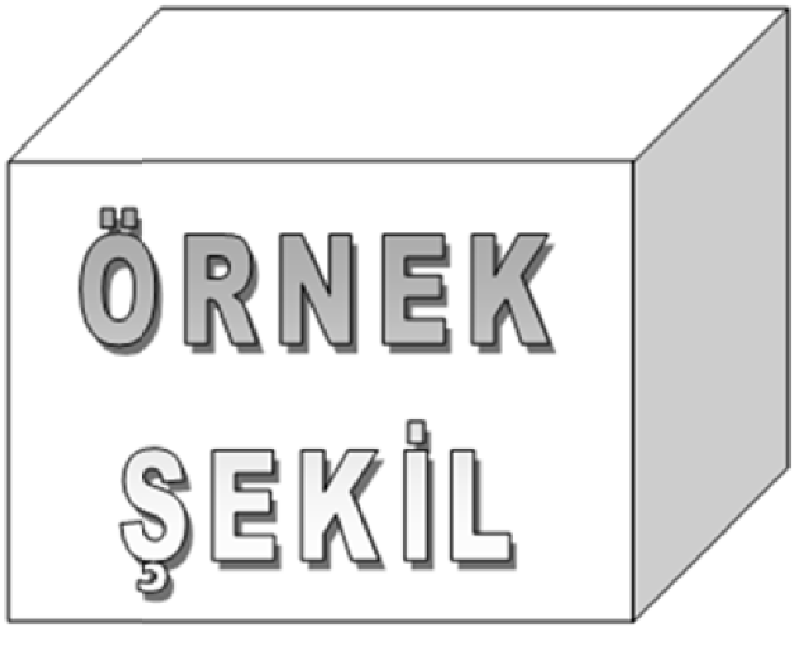
\includegraphics[scale=.3]{./fig/sekil1}
	% sekil1.eps: 0x0 pixel, 300dpi, 0.00x0.00 cm, bb=14 14 592 479
	\vspace{6pt}
	\caption{All tables and figures must be horizontally centered on the page.}
	\label{Figure2.1}
\end{figure}

%\begin{figure}
%	\begin{minipage}[b]{.5\linewidth}
%		\centering
%		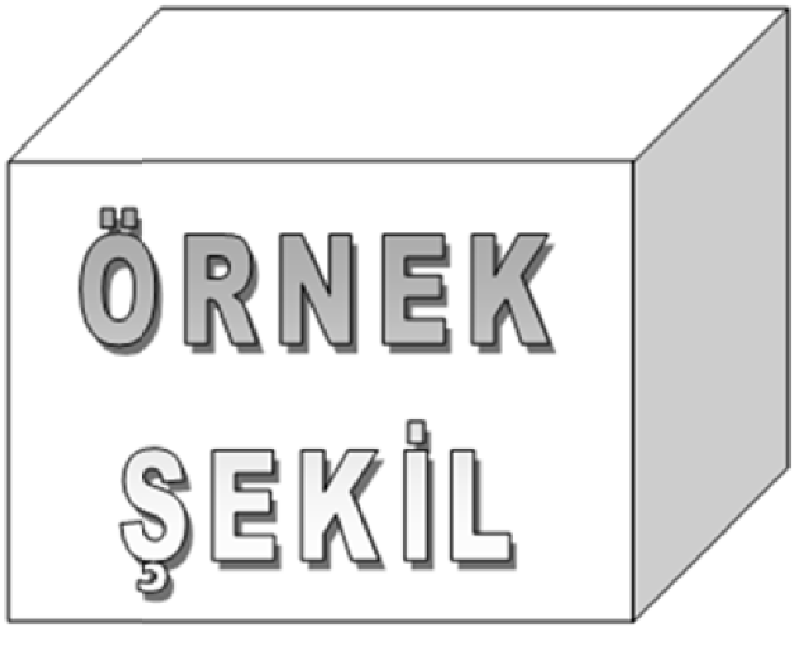
\includegraphics[scale=.2]{./fig/sekil1}
%		\subcaption{A subfigure}\label{Figure2.2a}
%	\end{minipage}
%	\begin{minipage}[b]{.5\linewidth}
%		\centering
%		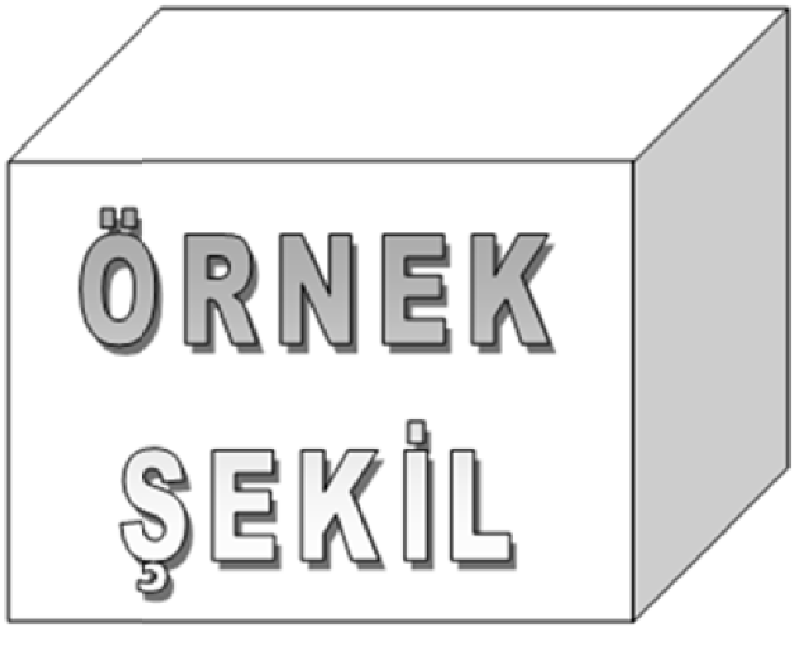
\includegraphics[scale=.2]{./fig/sekil1}
%		\subcaption{Another subfigure}\label{Figure2.2b}
%	\end{minipage}
%	\caption{A figure}\label{Figure2.2} % If no need a caption for main figure comment it out 
%\end{figure}
%%Figure letter: \subref{Figure2.2a}

%\begin{figure}
%	\begin{subfigure}[b]{.5\linewidth}
%		\centering
%		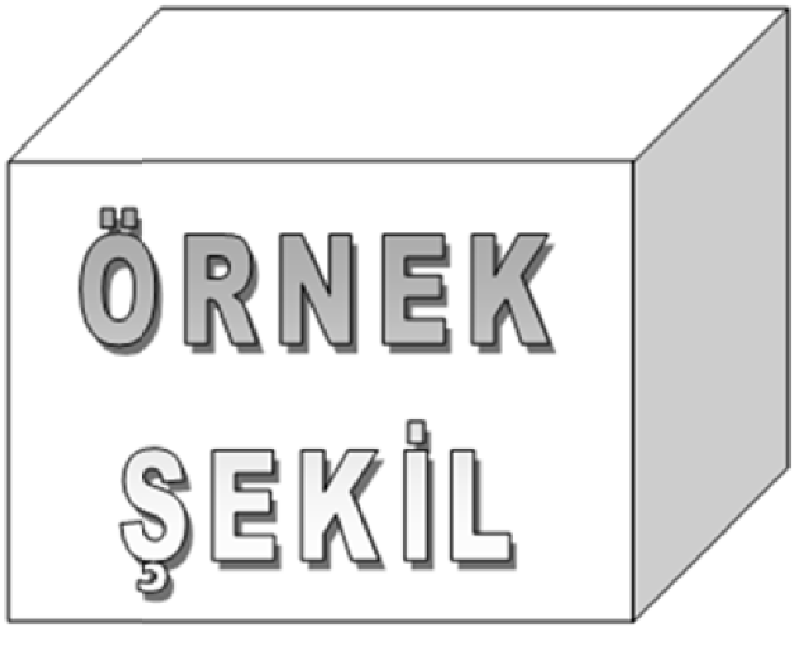
\includegraphics[scale=.2]{./fig/sekil1}
%		\caption{A subfigure}\label{Figure2.3a}
%	\end{subfigure}
%	\begin{subfigure}[b]{.5\linewidth}
%		\centering
%		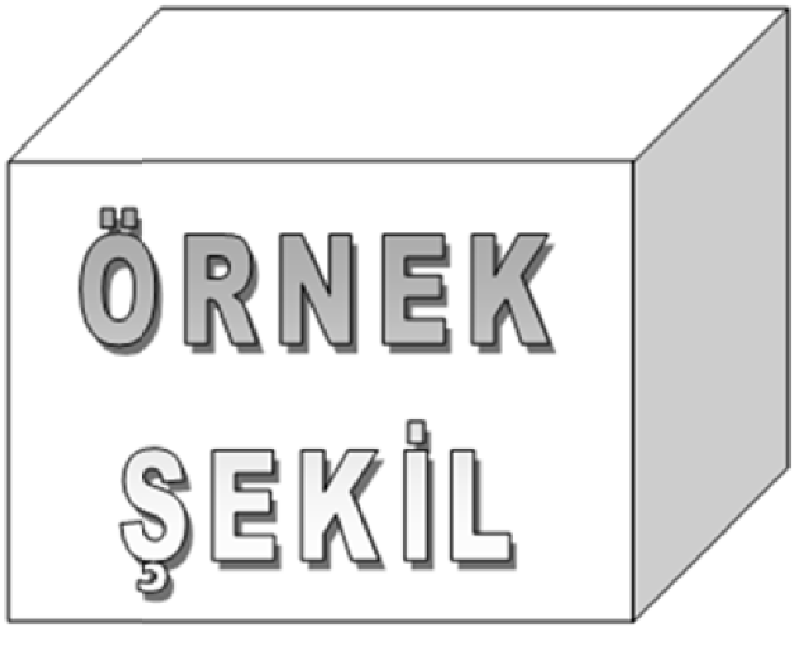
\includegraphics[scale=.2]{./fig/sekil1}
%		\caption{Another subfigure}\label{Figure2.3b}
%	\end{subfigure}
%	\caption{A figure}\label{Figure2.3}
%\end{figure}

% Subfigure example with proper LOF usage - SBÖ
\begin{figure}[h]
	\centering
	\begin{subfigure}{.8\textwidth}
		\centering
		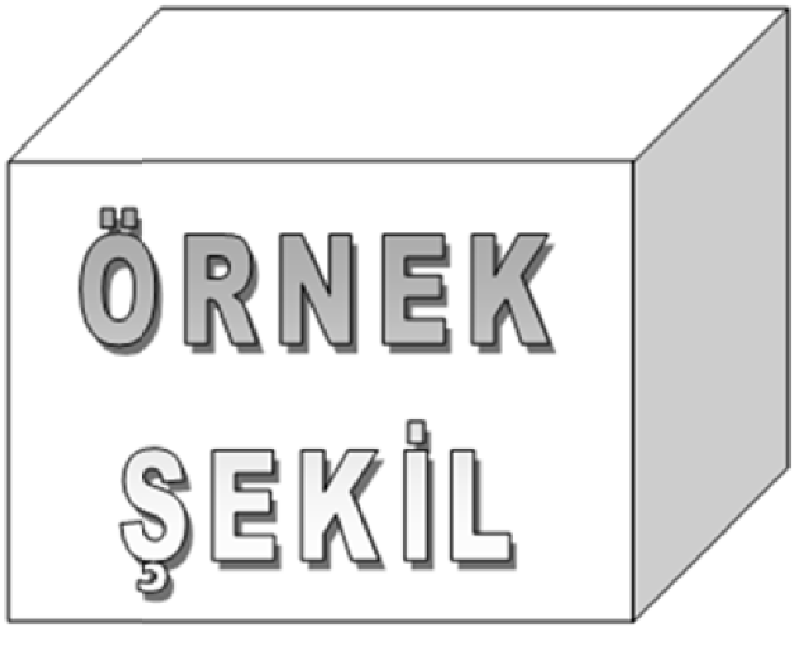
\includegraphics[scale=.3]{./fig/sekil1}
		\firstsubcaption{First subcaption of the subfigure.}
		\label{Figure2.2a}
	\end{subfigure}
	\begin{subfigure}{.8\textwidth}
		\centering
		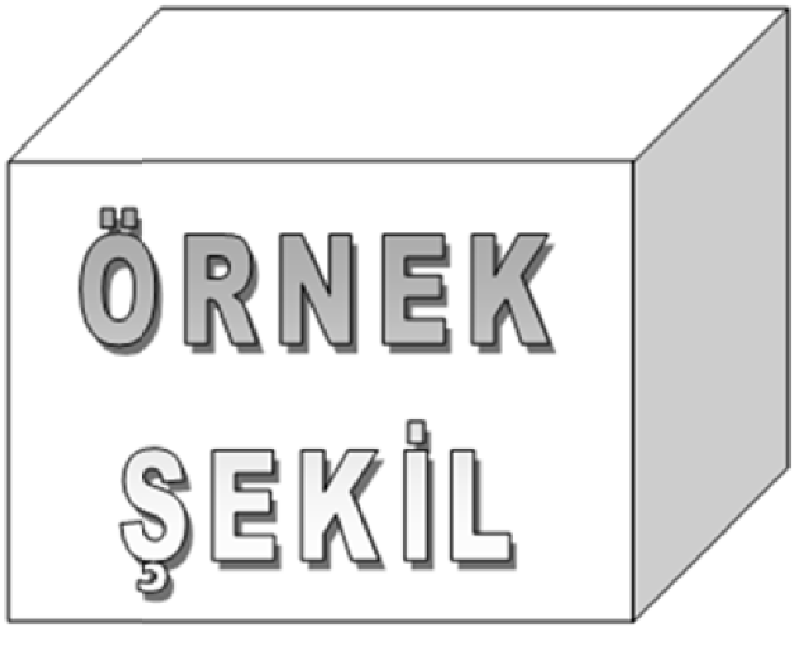
\includegraphics[scale=.3]{./fig/sekil1}
		\nextsubcaption{Second subcaption of the subfigure.}
		\label{Figure2.2b}
	\end{subfigure}
    \caption{An example of subfigure main caption.}\label{Figure2.2}
\end{figure}

%\begin{figure}
%	\centering     % not \center
%	\subcaption[]{Another subfigure}{\label{fig:a}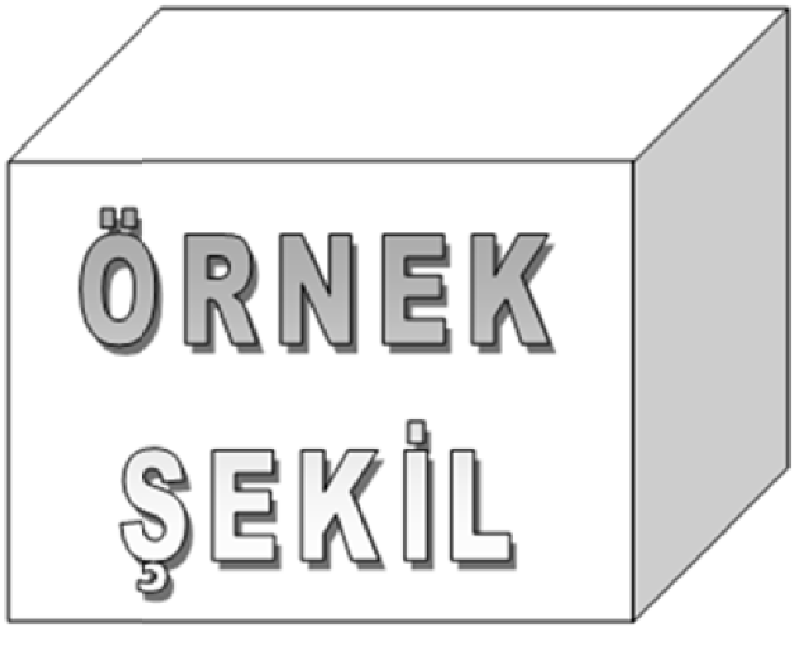
\includegraphics[scale=.2]{./fig/sekil1}}
%	\subcaption[]{Another subfigure}{\label{fig:b}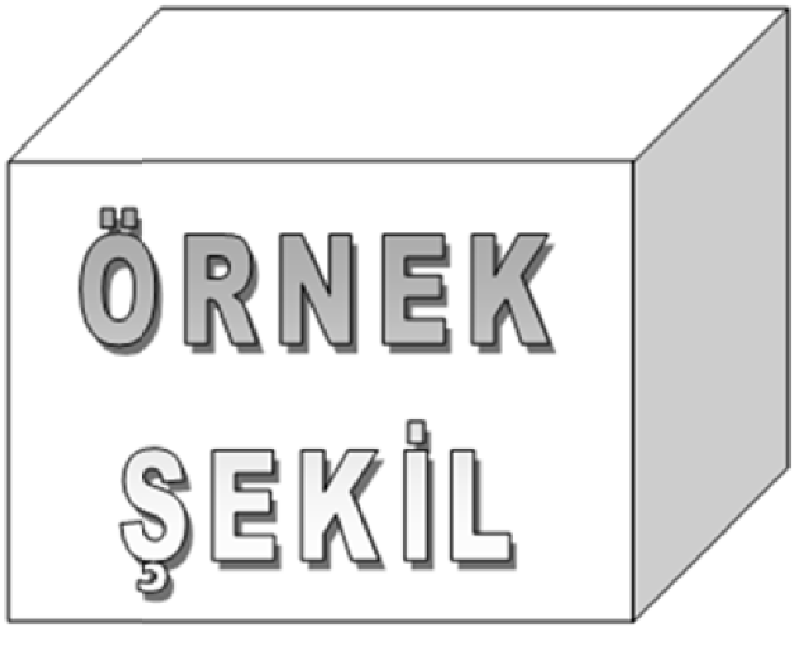
\includegraphics[scale=.2]{./fig/sekil1}}
%	%\caption{(a) this is fig 1 (b) this is fig 2.}
%	\label{L50}
%\end{figure}

In Figure \ref{Figure2.2}, sed diam nonumy eirmod tempor invidunt ut labore et dolore magna aliquyam erat, sed diam voluptua. At vero eos et accusam et justo duo dolores et ea rebum. Lorem ipsum dolor sit amet, consetetur sadipscing elitr, sed diam nonumy eirmod tempor invidunt ut labore et dolore magna aliquyam erat, sed diam voluptua. At vero eos et accusam et justo duo dolores et ea rebum. At vero eos et accusam et justo duo dolores et ea rebum. At vero eos et accusam et justo duo dolores et ea rebum. At vero eos et accusam et justo duo dolores et ea rebum. At vero eos et accusam et justo duo dolores et ea rebum. At vero eos et accusam et justo duo dolores et ea rebum. At vero eos et accusam et justo duo dolores et ea rebum in Figure \ref{Figure2.2a}.

\begin{figure}
	\centering
	
\includegraphics[width=10cm,keepaspectratio=true]{./fig/sekil2}
	% sekil2.eps: 0x0 pixel, 300dpi, 0.00x0.00 cm, bb=14 14 818 556
	\vspace{3pt}
	\caption{Example figure.}
	\label{Figure2.3}
\end{figure}
\vspace{-6pt}
\section{Landscape-oriented, full-page figure}

Lorem ipsum dolor sit amet, consetetur sadipscing elitr, sed diam nonumy eirmod tempor invidunt ut labore et dolore magna aliquyam erat, sed diam voluptua. At vero eos et accusam et justo duo dolores et ea rebum (Figure \ref{Figure2.3}). Lorem ipsum dolor sit amet, consetetur sadipscing elitr, sed diam nonumy eirmod tempor invidunt ut labore et dolore magna aliquyam erat, sed diam voluptua. At vero eos et accusam et justo duo dolores et ea rebum. 

Lorem ipsum dolor sit amet, consetetur sadipscing elitr, sed diam nonumy eirmod tempor invidunt ut labore et dolore magna aliquyam erat, sed diam voluptua. At vero eos et accusam et justo duo dolores et ea rebum. Lorem ipsum dolor sit amet, consetetur sadipscing elitr, sed diam nonumy eirmod tempor invidunt ut labore et dolore magna aliquyam erat, sed diam voluptua. At vero eos et accusam et justo duo dolores et ea rebum. Lorem ipsum dolor sit amet, consetetur sadipscing elitr, sed diam nonumy eirmod tempor invidunt ut labore et dolore magna aliquyam erat, sed diam voluptua. At vero eos et accusam et justo duo dolores et ea rebum \cite{Deci_Ryan_1990}. 

Lorem ipsum dolor sit amet, consetetur sadipscing elitr, sed diam nonumy eirmod tempor invidunt ut labore et dolore magna aliquyam erat, sed diam voluptua. At vero eos et accusam et justo duo dolores et ea rebum. Lorem ipsum dolor sit amet, consetetur sadipscing elitr, sed diam nonumy eirmod tempor invidunt ut labore et dolore magna aliquyam erat, sed diam voluptua. At vero eos et accusam et justo duo dolores et ea rebum. Lorem ipsum dolor sit amet, consetetur sadipscing elitr, sed diam nonumy eirmod tempor invidunt ut labore et dolore magna aliquyam erat, sed diam voluptua. At vero eos et accusam et justo duo dolores et ea rebum. Lorem ipsum dolor sit amet, consetetur sadipscing elitr, sed diam nonumy eirmod tempor invidunt ut labore et dolore magna aliquyam erat, sed diam voluptua. At vero eos et accusam et justo duo dolores et ea rebum \cite{lepichon}.

% Change margins on the fly to reset the page margins to one inch - SBÖ
\newenvironment{changemargin}[4]{
	\begin{list}{}{
			\setlength{\voffset}{#1}
			\setlength{\oddsidemargin}{#2}
			\setlength{\evensidemargin}{#3}
			\setlength{\textheight}{#3}
		}
		\item[] ~ \par
		% Get rid of the extra space inserted by the previous line
		%\vspace*{-2em}
	}{
	\end{list}
}

% All the figures and also odd page figures normally face inside the thesis, however the rule requires figures always face to the right. - SBÖ
% Figures on landscape pages has to be centered and facing to the right (ITU) - SBÖ
\begin{landscape}
	\thispagestyle{empty} %Remove the bottom page numbering
%	\begin{changemargin}{-0.4mm}{0mm}{0mm} %Set all the margins to zero - SBÖ
	%\thispagestyle{lscape}
	\vspace*{5mm}
	\begin{figure*}[ht]
		\centering
		%\begin{tabular}{@{}cc@{}}
		
\includegraphics[scale=.41,keepaspectratio=true]{./fig/sekil3} %&
		%
\includegraphics[width=50mm]{./fig/sekil3}
		%\end{tabular}                                       
		\caption{Landscape-oriented, full-page figure.}
		\label{Figure2.4}
	\end{figure*}
	
% Set the page number on the right side for odd numbered pages
      \begin{tikzpicture}[remember picture, overlay]
		\node[xshift=-25mm+148.5mm, yshift=17mm-210mm+15mm] (number) at (current page text area.east) {\thepage};
	  \end{tikzpicture}
	  
%\end{changemargin}
\end{landscape}

% All the figures and also even page figures normally face inside the thesis, however the rule requires figures always face to the right. - SBÖ
% Figures on landscape pages has to be centered and facing to the right (ITU) - SBÖ
\begin{landscape}
	\thispagestyle{empty} % Remove the bottom page numbering
%	\begin{changemargin}{-0.4mm}{0mm}{0mm} %Set all the margins to zero - SBÖ
		%\thispagestyle{lscape}

		\vspace*{20mm}
		\begin{figure*}[ht]
			\centering
			%\begin{tabular}{@{}cc@{}}
				
\includegraphics[scale=.41,keepaspectratio=true]{./fig/sekil3} %&
				%
\includegraphics[width=50mm]{./fig/sekil3}
			%\end{tabular}                                       
			\caption{Landscape-oriented, full-page figure.}
			\label{Figure2.5}
		\end{figure*}
	   
% Set the page number on the left side for even numbered pages
		%\begin{tikzpicture}[remember picture, overlay]
		% \node[xshift=-25mm+148.5mm, yshift=-1mm-15mm, rotate=180] (number) at (current page text area.east) {\thepage};
		%\end{tikzpicture}
		
% Set the page number on the right side for even numbered pages as well
		\begin{tikzpicture}[remember picture, overlay]
		 \node[xshift=-25mm+148.5mm, yshift=17mm-210mm] (number) at (current page text area.east) {\thepage};
		\end{tikzpicture}
		
%	\end{changemargin}
\end{landscape}

%\newpage
\section{Table Citations and Table Example}

Lorem ipsum dolor sit amet, consetetur sadipscing elitr, sed diam nonumy eirmod tempor invidunt ut labore et dolore magna aliquyam erat, sed diam voluptua. At vero eos et accusam et justo duo dolores et ea rebum. Stet clita kasd gub rgren, no sea takimata sanctus est Lorem ipsum dolor sit amet, consetetur sadipscing elitr, sed diam nonumy eirmod tempor invidunt ut lab ore sit et dolore magna.

\begin{table*}[h]
	{\setlength{\tabcolsep}{14pt}
		\caption{Table with single row and centered columns.}
		\begin{center}
			\vspace{-6mm}
			\begin{tabular}{cccc}
				\hline \\[-2.45ex] \hline \\[-2.1ex]
				Column A & Column B & Column C & Column D \\
				\hline \\[-1.8ex]
				Row A & Row A & Row A & Row A \\
				Row B & Row B & Row B & Row B \\
				Row C & Row C & Row C & Row C \\
				\hline
			\end{tabular}
			\vspace{-6mm}
		\end{center}
		\label{Table2.1}}
\end{table*}

As seen in Table \ref{Table2.1}, lorem ipsum dolor sit amet, consetetur sadipscing elitr, sed diam nonumy eirmod tempor invidunt ut labore et dolore magna aliquyam erat, sed diam voluptua. At vero eos et accusam et justo duo dolores et ea rebum. Stet clita kasd gub rgren, no sea takimata sanctus est Lorem ipsum dolor sit amet, consetetur sadipscing elitr, sed diam nonumy eirmod tempor invidunt ut lab ore sit et dolore magna.

\begin{table*}[h]
	{\setlength{\tabcolsep}{14pt}
		\caption{Table captions must be ended with a full stop.}
		\begin{center}
			\vspace{-6mm}
			\begin{tabular}{cccc}
				\hline \\[-2.45ex] \hline \\[-2.1ex]
				Column A & Column B & Column C & Column D \\
				\hline \\[-1.8ex]
				Row A & Row A & Row A & Row A \\
				Row B & Row B & Row B & Row B \\
				Row C & Row C & Row C & Row C \\
				\hline
			\end{tabular}
			\vspace{-6mm}
		\end{center}
		\label{Table2.2}}
\end{table*}

Lorem ipsum dolor sit amet, consetetur sadipscing elitr, sed diam nonumy eirmod tempor invidunt ut labore et dolore magna aliquyam erat, sed diam voluptua. At vero eos et accusam et justo duo dolores et ea rebum, as seen in Table \ref{Table2.2}. 

Lorem ipsum dolor sit amet, consetetur sadipscing elitr, sed diam nonumy eirmod tempor invidunt ut labore et dolore magna aliquyam erat, sed diam voluptua. At vero eos et accusam et justo duo dolores et ea rebum. Stet clita kasd gub rgren, no sea takimata sanctus est Lorem ipsum dolor sit amet, consetetur sadipscing elitr, sed diam nonumy eirmod tempor invidunt ut lab ore sit et dolore magna. Lorem ipsum dolor sit amet, consetetur sadipscing elitr, sed diam nonumy eirmod tempor invidunt ut labore et dolore magna aliquyam erat, sed diam voluptua. At vero eos et accusam et justo duo dolores et ea rebum \cite{Roberts_Jackson_1991}. 

\section{Landscape-oriented, full-page table}

Lorem ipsum dolor sit amet, consetetur sadipscing elitr, sed diam nonumy eirmod tempor invidunt ut labore et dolore magna aliquyam erat, sed diam voluptua. At vero eos et accusam et justo duo dolores et ea rebum. Stet clita kasd gub rgren, no sea takimata sanctus est Lorem ipsum dolor sit amet, consetetur sadipscing elitr, sed diam nonumy eirmod tempor invidunt ut lab ore sit et dolore magna.

% ---------------------------------------------------------------- %
% Page numbers must be on the bottom-middle of short side (when    %
% portrait-oriented), or bottom-middle of long side (when	       %
% landscape-oriented)						                       %
% ---------------------------------------------------------------- %
% Odd page landscape table and page numbering - SBÖ		
\begin{landscape}
	\thispagestyle{empty}
%	\vspace*{-6mm}
%	\begin{changemargin}{0.4mm}{0mm}{0mm} %Set all the margins to zero - SBÖ
	\begin{table*}[htb!]
		{\setlength{\tabcolsep}{14pt}
			%\hspace*{5mm}
			%\vspace*{-6mm}
			\caption{Prof. Dr. Galip TEPEHAN \,\, Captioning in landscape-oriented pages:
				the most important aspect is to align the lines horizontally.}
			\begin{center}
				\vspace{-6mm}
				\begin{tabular}{lccrrrrr}
					\hline\hline
					\multirow{2}{*}{Parametre} & \multirow{2}{*}{Column 2} & \multirow{2}{*}{Column 3} & \multicolumn{3}{c|}{Column 4} & \multicolumn{2}{c}{Column 5}\\ \cline{4-8}
					& & & Subcolumn & Subcolumn & Subcolumn & Subcolumn & Subcolumn\\
					\hline
					Row 1 & -7.680442 & 7.6986348 & 0.00 & 0.00 & 0.00 & 12 & 12 \\
					Row 2 & 140 & - & 0.50 & 0.00 & 0.00 & 0 & 0 \\
					Row 3 & 37.174357 & 37.16192697 & 0.00 & 0.00 & 0.00 & 0 & 24 \\
					Row 4 & 140 & - & 0.50 & 0.00 & 0.00 & 0 & 0 \\
					Row 5 & 37.174357 & 37.16192697 & 0.00 & 0.00 & 0.00 & 0 & 24 \\
					Row 6 & 140 & - & 0.50 & 0.00 & 0.00 & 0 & 0 \\
					Row 7 & 37.174357 & 37.16192697 & 0.00 & 0.00 & 0.00 & 0 & 24 \\
					Row 8 & 140 & - & 0.50 & 0.00 & 0.00 & 0 & 0 \\
					Row 9 & 37.174357 & 37.16192697 & 0.00 & 0.00 & 0.00 & 0 & 24 \\
					Row 10 & 140 & - & 0.50 & 0.00 & 0.00 & 0 & 0 \\
					Row 11 & 37.174357 & 37.16192697 & 0.00 & 0.00 & 0.00 & 0 & 24 \\
					Row 12 & 140 & - & 0.50 & 0.00 & 0.00 & 0 & 0 \\
					Row 13 & 37.174357 & 37.16192697 & 0.00 & 0.00 & 0.00 & 0 & 24 \\
					Row 14 & 140 & - & 0.50 & 0.00 & 0.00 & 0 & 0 \\
					Row 15 & 37.174357 & 37.16192697 & 0.00 & 0.00 & 0.00 & 0 & 24 \\
					\hline
				\end{tabular}
			\end{center}
			\begin{center}
				\label{Table2.3}
			\end{center}
		}
	\end{table*}
% Set the page number on the right side for odd numbered pages
		\begin{tikzpicture}[remember picture,overlay]
		\node[xshift=-10mm+148.5mm, yshift=2mm-210mm+30mm] (number) at (current page text area.east) {\thepage};
		\end{tikzpicture}
%   \end{changemargin}
\end{landscape}

% ---------------------------------------------------------------- %
% Page numbers must be on the bottom-middle of short side (when    %
% portrait-oriented), or bottom-middle of long side (when	       %
% landscape-oriented)						                       %
% ---------------------------------------------------------------- %
% Even page landscape table and page numbering - SBÖ		
\begin{landscape}
	\thispagestyle{empty}
	%\vspace*{-6mm}
%	\begin{changemargin}{0.4mm}{0mm}{0mm} %Set all the margins to zero - SBÖ
		\begin{table*}[htb!]
			{\setlength{\tabcolsep}{14pt}
				%\hspace*{5mm}
				%\vspace*{-6mm}
				\caption{Prof. Dr. Galip TEPEHAN \,\, Captioning in landscape-oriented pages:
					the most important aspect is to align the lines horizontally.}
				\begin{center}
					\vspace{-6mm}
					\begin{tabular}{lccrrrrr}
						\hline\hline
						\multirow{2}{*}{Parametre} & \multirow{2}{*}{Column 2} & \multirow{2}{*}{Column 3} & \multicolumn{3}{c|}{Column 4} & \multicolumn{2}{c}{Column 5}\\ \cline{4-8}
						& & & Subcolumn & Subcolumn & Subcolumn & Subcolumn & Subcolumn\\
						\hline
						Row 1 & -7.680442 & 7.6986348 & 0.00 & 0.00 & 0.00 & 12 & 12 \\
						Row 2 & 140 & - & 0.50 & 0.00 & 0.00 & 0 & 0 \\
						Row 3 & 37.174357 & 37.16192697 & 0.00 & 0.00 & 0.00 & 0 & 24 \\
						Row 4 & 140 & - & 0.50 & 0.00 & 0.00 & 0 & 0 \\
						Row 5 & 37.174357 & 37.16192697 & 0.00 & 0.00 & 0.00 & 0 & 24 \\
						Row 6 & 140 & - & 0.50 & 0.00 & 0.00 & 0 & 0 \\
						Row 7 & 37.174357 & 37.16192697 & 0.00 & 0.00 & 0.00 & 0 & 24 \\
						Row 8 & 140 & - & 0.50 & 0.00 & 0.00 & 0 & 0 \\
					\end{tabular}
				\end{center}
				\begin{center}
					\label{Table2.4}
				\end{center}
			}
		\end{table*}
% Set the page number on the right side for even numbered pages
		\begin{tikzpicture}[remember picture,overlay]
		\node[xshift=-25mm+148.5mm, yshift=2mm-210mm+15mm] (number) at (current page text area.east) {\thepage};
		\end{tikzpicture}
%	\end{changemargin}
\end{landscape}

\begin{table}[!htbp] \centering
	\caption{ Neighborhoods Visited }
	\vspace{-3mm}
	\label{}
	\begin{tabular}{@{\extracolsep{5pt}} llrrr} 
	\\[-1.8ex]\hline 
		\hline \\[-1.8ex] 
		\multicolumn{1}{c}{Variable} & \multicolumn{1}{c}{Values} & \multicolumn{1}{c}{Count} & \multicolumn{1}{c}{\%} & \multicolumn{1}{c}{Cum. \%} \\
		\hline \\[-1.8ex] 
		\multirow{ 4 }{*}{ visit }  &  FALSE  &  2  &  33.33  &  33.33  \\
		\hhline{}  &  TRUE  &  3  &  50.00  &  83.33  \\
		\hhline{}  &  NA  &  1  &  16.67  &  100.00  \\
	    \hhline{}  &  Total  &  6  &  100.00  &    \\
		\hline \\[-1.8ex] 
	\end{tabular}
\end{table}

% Multi-page longtable example spreading couple of pages - SBÖ
\begin{center}
	\begin{longtable}{ccc}
		%Here is the caption, the stuff in [] is the table of contents entry,
		%the stuff in {} is the title that will appear on the first page of the
		%table.
		\caption[Feasible triples for a highly variable Grid]{Feasible triples
			for highly variable Grid, MLMMH.} \label{Table2.6} \vspace{-1.75mm}\\
		%This is the header for the first page of the table...
		\hline\\[-2.45ex] \hline \\[-1.8ex] % Distancing of the hlines adjausted from the text 
		\multicolumn{1}{c}{{Time (s)}} &
		\multicolumn{1}{c}{{Triple chosen}} &
		\multicolumn{1}{c}{{Other feasible triples}} \\[0.5ex] \hline
		\\[-1.8ex]
		\endfirsthead
		
		%This is the header for the remaining page(s) of the table...
		\multicolumn{3}{c}{{\tablename} \textbf{\thetable{}} \textbf{(continued) :} Feasible triples
			for highly variable Grid, MLMMH.} \\[0.5ex]
		\hline\\[-2.45ex] \hline \\[-1.8ex]
		\multicolumn{1}{c}{{Time (s)}} &
		\multicolumn{1}{c}{{Triple chosen}} &
		\multicolumn{1}{c}{{Other feasible triples}} \\[0.5ex] \hline
		\\[-1.8ex]
		\endhead
		
		%This is the footer for all pages except the last page of the table...
		%\multicolumn{3}{l}{{Continued on Next Page\ldots}} \\
		\\[-1.8ex] \hline
		\endfoot
		
		%This is the footer for the last page of the table...
		\\[-1.8ex] \hline
		\endlastfoot
		
		%Now the data...
		0      & (1, 11, 13725) & (1, 12, 10980), (1, 13, 8235), (2, 2, 0), (3, 1, 0) \\
		2745   & (1, 12, 10980) & (1, 13, 8235), (2, 2, 0), (2, 3, 0), (3, 1, 0) \\
		5490   & (1, 12, 13725) & (2, 2, 2745), (2, 3, 0), (3, 1, 0) \\
		8235   & (1, 12, 16470) & (1, 13, 13725), (2, 2, 2745), (2, 3, 0), (3, 1, 0) \\
		% <data removed>
		164700 & (1, 13, 13725) & (2, 2, 2745), (2, 3, 0), (3, 1, 0) \\
		0      & (1, 11, 13725) & (1, 12, 10980), (1, 13, 8235), (2, 2, 0), (3, 1, 0) \\
		2745   & (1, 12, 10980) & (1, 13, 8235), (2, 2, 0), (2, 3, 0), (3, 1, 0) \\
		5490   & (1, 12, 13725) & (2, 2, 2745), (2, 3, 0), (3, 1, 0) \\
		8235   & (1, 12, 16470) & (1, 13, 13725), (2, 2, 2745), (2, 3, 0), (3, 1, 0) \\
		% <data removed>
		164700 & (1, 13, 13725) & (2, 2, 2745), (2, 3, 0), (3, 1, 0) \\
		0      & (1, 11, 13725) & (1, 12, 10980), (1, 13, 8235), (2, 2, 0), (3, 1, 0) \\
		2745   & (1, 12, 10980) & (1, 13, 8235), (2, 2, 0), (2, 3, 0), (3, 1, 0) \\
		5490   & (1, 12, 13725) & (2, 2, 2745), (2, 3, 0), (3, 1, 0) \\
		8235   & (1, 12, 16470) & (1, 13, 13725), (2, 2, 2745), (2, 3, 0), (3, 1, 0) \\
		% <data removed>
		164700 & (1, 13, 13725) & (2, 2, 2745), (2, 3, 0), (3, 1, 0) \\
		0      & (1, 11, 13725) & (1, 12, 10980), (1, 13, 8235), (2, 2, 0), (3, 1, 0) \\
		2745   & (1, 12, 10980) & (1, 13, 8235), (2, 2, 0), (2, 3, 0), (3, 1, 0) \\
		5490   & (1, 12, 13725) & (2, 2, 2745), (2, 3, 0), (3, 1, 0) \\
		8235   & (1, 12, 16470) & (1, 13, 13725), (2, 2, 2745), (2, 3, 0), (3, 1, 0) \\
		% <data removed>
		164700 & (1, 13, 13725) & (2, 2, 2745), (2, 3, 0), (3, 1, 0) \\
		0      & (1, 11, 13725) & (1, 12, 10980), (1, 13, 8235), (2, 2, 0), (3, 1, 0) \\
		2745   & (1, 12, 10980) & (1, 13, 8235), (2, 2, 0), (2, 3, 0), (3, 1, 0) \\
		5490   & (1, 12, 13725) & (2, 2, 2745), (2, 3, 0), (3, 1, 0) \\
		8235   & (1, 12, 16470) & (1, 13, 13725), (2, 2, 2745), (2, 3, 0), (3, 1, 0) \\
		% <data removed>
		164700 & (1, 13, 13725) & (2, 2, 2745), (2, 3, 0), (3, 1, 0) \\
		0      & (1, 11, 13725) & (1, 12, 10980), (1, 13, 8235), (2, 2, 0), (3, 1, 0) \\
		2745   & (1, 12, 10980) & (1, 13, 8235), (2, 2, 0), (2, 3, 0), (3, 1, 0) \\
		5490   & (1, 12, 13725) & (2, 2, 2745), (2, 3, 0), (3, 1, 0) \\
		8235   & (1, 12, 16470) & (1, 13, 13725), (2, 2, 2745), (2, 3, 0), (3, 1, 0) \\
		% <data removed>
		164700 & (1, 13, 13725) & (2, 2, 2745), (2, 3, 0), (3, 1, 0) \\
		0      & (1, 11, 13725) & (1, 12, 10980), (1, 13, 8235), (2, 2, 0), (3, 1, 0) \\
		2745   & (1, 12, 10980) & (1, 13, 8235), (2, 2, 0), (2, 3, 0), (3, 1, 0) \\
		5490   & (1, 12, 13725) & (2, 2, 2745), (2, 3, 0), (3, 1, 0) \\
		8235   & (1, 12, 16470) & (1, 13, 13725), (2, 2, 2745), (2, 3, 0), (3, 1, 0) \\ \noalign{\penalty-5000}
		% <data removed>
		164700 & (1, 13, 13725) & (2, 2, 2745), (2, 3, 0), (3, 1, 0) \\
		0      & (1, 11, 13725) & (1, 12, 10980), (1, 13, 8235), (2, 2, 0), (3, 1, 0) \\
		2745   & (1, 12, 10980) & (1, 13, 8235), (2, 2, 0), (2, 3, 0), (3, 1, 0) \\
		5490   & (1, 12, 13725) & (2, 2, 2745), (2, 3, 0), (3, 1, 0) \\
		8235   & (1, 12, 16470) & (1, 13, 13725), (2, 2, 2745), (2, 3, 0), (3, 1, 0) \\
		% <data removed>
		164700 & (1, 13, 13725) & (2, 2, 2745), (2, 3, 0), (3, 1, 0) \\
		0      & (1, 11, 13725) & (1, 12, 10980), (1, 13, 8235), (2, 2, 0), (3, 1, 0) \\
		2745   & (1, 12, 10980) & (1, 13, 8235), (2, 2, 0), (2, 3, 0), (3, 1, 0) \\
		5490   & (1, 12, 13725) & (2, 2, 2745), (2, 3, 0), (3, 1, 0) \\
		8235   & (1, 12, 16470) & (1, 13, 13725), (2, 2, 2745), (2, 3, 0), (3, 1, 0) \\
		% <data removed>
		164700 & (1, 13, 13725) & (2, 2, 2745), (2, 3, 0), (3, 1, 0) \\
		0      & (1, 11, 13725) & (1, 12, 10980), (1, 13, 8235), (2, 2, 0), (3, 1, 0) \\
		2745   & (1, 12, 10980) & (1, 13, 8235), (2, 2, 0), (2, 3, 0), (3, 1, 0) \\
		5490   & (1, 12, 13725) & (2, 2, 2745), (2, 3, 0), (3, 1, 0) \\
		8235   & (1, 12, 16470) & (1, 13, 13725), (2, 2, 2745), (2, 3, 0), (3, 1, 0) \\
		% <data removed>
		164700 & (1, 13, 13725) & (2, 2, 2745), (2, 3, 0), (3, 1, 0) \\
		0      & (1, 11, 13725) & (1, 12, 10980), (1, 13, 8235), (2, 2, 0), (3, 1, 0) \\
		2745   & (1, 12, 10980) & (1, 13, 8235), (2, 2, 0), (2, 3, 0), (3, 1, 0) \\
		5490   & (1, 12, 13725) & (2, 2, 2745), (2, 3, 0), (3, 1, 0) \\
		8235   & (1, 12, 16470) & (1, 13, 13725), (2, 2, 2745), (2, 3, 0), (3, 1, 0) \\
		% <data removed>
		164700 & (1, 13, 13725) & (2, 2, 2745), (2, 3, 0), (3, 1, 0) \\
		0      & (1, 11, 13725) & (1, 12, 10980), (1, 13, 8235), (2, 2, 0), (3, 1, 0) \\
		2745   & (1, 12, 10980) & (1, 13, 8235), (2, 2, 0), (2, 3, 0), (3, 1, 0) \\
		5490   & (1, 12, 13725) & (2, 2, 2745), (2, 3, 0), (3, 1, 0) \\
		8235   & (1, 12, 16470) & (1, 13, 13725), (2, 2, 2745), (2, 3, 0), (3, 1, 0) \\
		% <data removed>
		164700 & (1, 13, 13725) & (2, 2, 2745), (2, 3, 0), (3, 1, 0) \\
		0      & (1, 11, 13725) & (1, 12, 10980), (1, 13, 8235), (2, 2, 0), (3, 1, 0) \\
		2745   & (1, 12, 10980) & (1, 13, 8235), (2, 2, 0), (2, 3, 0), (3, 1, 0) \\
		5490   & (1, 12, 13725) & (2, 2, 2745), (2, 3, 0), (3, 1, 0) \\
		8235   & (1, 12, 16470) & (1, 13, 13725), (2, 2, 2745), (2, 3, 0), (3, 1, 0) \\
	\end{longtable}
\end{center}
%%%%%%%%%%%%%%%%%%%%%%%%%%%%%%%%%%%%%%%%%%%%%%%%%%%%%%%%%%%%%%%%%
\chapter{MAIN TEXT BODY}\label{ch:Ch3}
%%%%%%%%%%%%%%%%%%%%%%%%%%%%%%%%%%%%%%%%%%%%%%%%%%%%%%%%%%%%%%%%%
\vspace*{-12pt} % If no text above section, use this vspacing to lift the whole part to the proper starting point - SBÖ
\section{Body Texts}

Lorem ipsum dolor sit amet, consetetur sadipscing elitr, sed diam nonumy eirmod tempor invidunt ut labore et dolore magna aliquyam erat, sed diam voluptua. At vero eos et accusam et justo duo dolores et ea rebum. Stet clita kasd gub rgren, no sea takimata sanctus est Lorem ipsum dolor sit amet, consetetur sadipscing elitr, sed diam nonumy eirmod tempor invidunt ut lab ore sit et dolore magna.

Lorem ipsum dolor sit amet, consetetur sadipscing elitr, sed diam nonumy eirmod tempor invidunt ut labore et dolore magna aliquyam erat, sed diam voluptua. At vero eos et accusam et justo duo dolores et ea rebum. Stet clita kasd gub rgren, no sea takimata sanctus est Lorem ipsum dolor sit amet, consetetur sadipscing elitr, sed diam nonumy eirmod tempor invidunt ut lab ore sit et dolore magna.
 
\subsection{Page Margins}

Lorem ipsum dolor sit amet, consetetur sadipscing elitr, sed diam Lorem ipsum dolor sit amet, consetetur sadipscing elitr, sed diam nonumy eirmod tempor invidunt ut labore et dolore magna aliquyam erat, sed diam voluptua. At vero eos et accusam et justo duo dolores et ea rebum (Figure \ref{Figure3.1}).

The gap at the bottom of the page is 2.5 cm. 

Keeping more redundant space is incorrect. So, this gap should not be. Texts, tables, figures, etc. in the pages must be arranged considering this situation.

%\setitemize{leftmargin=2em} % Left margin given to the bullets - SBÖ
\begin{itemize}
	\setlength{\itemindent}{-0.35em} % Flush the bullets to the left - SBÖ
	\item{Figures, tables can be enlarged and be reduced.}
	\vspace{-3mm}
	\item{The explanations except from the first reference about the figure or table can be placed either before the figure/table or after.}
	\vspace{-3mm}
	\item{After referring to a figure or table it is placed to the closest and convenient location. Convenient location must be arranged considering the gap at the bottom of the page.}
\end{itemize}

\begin{figure}
%\begin{sidewaysfigure}
	\centering
	
\includegraphics[width=280pt,keepaspectratio=true]{./fig/sekil3}
	% sekil3.eps: 0x0 pixel, 300dpi, 0.00x0.00 cm, bb=14 14 1155 740
	\caption{Neuron cell, adapted from (\c{C}etin, 2003).}
	\label{Figure3.1}
%\end{sidewaysfigure}
\end{figure}

Lorem ipsum dolor sit amet, consetetur sadipscing elitr, sed diam nonumy eirmod tempor invidunt ut labore et dolore magna aliquyam erat, sed diam voluptua. At vero eos et accusam et justo duo dolores et ea rebum. Stet clita kasd gub rgren, no sea takimata sanctus est Lorem ipsum dolor sit amet, consetetur sadipscing elitr, sed diam nonumy eirmod tempor invidunt ut lab ore sit et dolore magna.

At vero eos et accusam et justo duo dolores et ea rebum. Stet clita kasd gub rgren, no sea takimata sanctus est Lorem ipsum dolor sit amet, consetetur sadipscing elitr, sed diam nonumy eirmod tempor invidunt ut lab ore sit et dolore magna.

Lorem ipsum dolor sit amet, consetetur sadipscing elitr, sed diam nonumy eirmod tempor invidunt ut labore et dolore magna aliquyam erat, sed diam voluptua. At vero eos et accusam et justo duo dolores et ea rebum. Stet clita kasd gub rgren, no sea takimata sanctus est Lorem ipsum dolor sit amet, consetetur sadipscing elitr, sed diam nonumy eirmod tempor invidunt ut lab ore sit et dolore magna.

\subsection{Equations}

Lorem ipsum dolor sit amet, consetetur sadipscing elitr, sed diam nonumy eirmod tempor invidunt ut labore et dolore magna aliquyam erat, sed diam voluptua. At vero eos et accusam et justo duo dolores et ea rebum. Stet clita kasd gub rgren, no sea takimata sanctus est  Lorem ipsum dolor sit amet, consetetur sadipscing elitr, sed diam nonumy eirmod tempor invidunt ut lab  ore sit et dolore magna equation (\ref{Eq3.1}).
\begin{equation}
y_{t} = \phi_{1} y_{t-1} + \epsilon_{t}
\label{Eq3.1}
\end{equation}
Lorem ipsum dolor sit amet, consetetur sadipscing elitr, sed diam nonumy eirmod tempor invidunt ut labore et dolore magna aliquyam erat, sed diam voluptua. At vero eos et accusam et justo duo dolores et ea rebum. Stet clita kasd gub rgren, no sea takimata sanctus est Lorem ipsum dolor sit amet, consetetur sadipscing elitr, sed diam nonumy eirmod tempor invidunt ut lab ore sit et dolore magna.
% Subequation example - SBÖ
\vskip -24pt
\begin{subequations}
	\begin{gather}
	R_0 = 0 \label{Eq3.2a}\\
	N_0 = 0 \label{Eq3.2b}
	\end{gather}
	\label{Eq3.2ab}
\end{subequations}
\vskip -24pt
Each parameter is described, as seen in equation \eqref{Eq3.1}, or in \ref{Eq3.1}. Lorem ipsum dolor sit amet, consetetur sadipscing elitr, sed diam nonumy eirmod tempor invidunt ut labore et dolore equation \ref{Eq3.1}’in magna aliquyam erat Equation \eqref{Eq3.2ab} into Equation \eqref{Eq3.2a} and Equation \eqref{Eq3.2b}.

\subsection{Process based model: SWAT}

Lorem ipsum dolor sit amet, consetetur sadipscing elitr, sed diam nonumy eirmod tempor invidunt ut labore et dolore magna aliquyam erat, sed diam voluptua. At vero eos et accusam et justo duo dolores et ea rebum. Stet clita kasd gub rgren, no sea takimata sanctus est Lorem ipsum dolor sit amet, consetetur sadipscing elitr, sed diam nonumy eirmod tempor invidunt ut lab ore sit et dolore magna.

Lorem ipsum dolor sit amet, consetetur sadipscing elitr, sed diam nonumy eirmod tempor invidunt ut labore et dolore magna aliquyam erat, sed diam voluptua. At vero eos et accusam et justo duo dolores et ea rebum. Stet clita kasd gub rgren, no sea takimata sanctus est Lorem ipsum dolor sit amet, consetetur sadipscing elitr, sed diam nonumy eirmod tempor invidunt ut lab ore sit et dolore magna.

\begin{figure}
	\centering
	
\includegraphics[width=250pt,keepaspectratio=true]{./fig/sekil3}
	% sekil3.eps: 0x0 pixel, 300dpi, 0.00x0.00 cm, bb=14 14 1155 740
	\caption{For a multi-line figure captions, it is important that all the lines of the caption are aligned.}
	\label{Figure3.2}
\end{figure}

\subsection{Multi variable analysis}

Lorem ipsum dolor sit amet, consetetur sadipscing elitr, sed diam nonumy eirmod tempor invidunt ut labore et dolore magna aliquyam erat, sed diam voluptua. At vero eos et accusam et justo duo dolores et ea rebum. Stet clita kasd gub rgren, no sea takimata sanctus est Lorem ipsum dolor sit amet, consetetur sadipscing elitr, sed diam nonumy eirmod tempor invidunt ut lab ore sit et dolore magna (\ref{Eq3.2}). Lorem ipsum dolor sit amet, consetetur sadipscing elitr, sed diam nonumy eirmod tempor invidunt ut labore et dolore magna aliquyam erat, sed diam voluptua. At vero eos et accusam et justo duo dolores et ea rebum. Lorem ipsum dolor sit amet, consetetur sadipscing elitr, sed diam nonumy eirmod tempor invidunt ut labore et dolore magna aliquyam erat, sed diam voluptua. At vero eos et accusam et justo duo dolores et ea rebum. Lorem ipsum dolor sit amet, consetetur sadipscing elitr, sed diam nonumy eirmod tempor invidunt ut labore et dolore magna aliquyam erat, sed diam voluptua. At vero eos et accusam et justo duo dolores et ea rebum.

\begin{figure}
	\centering
	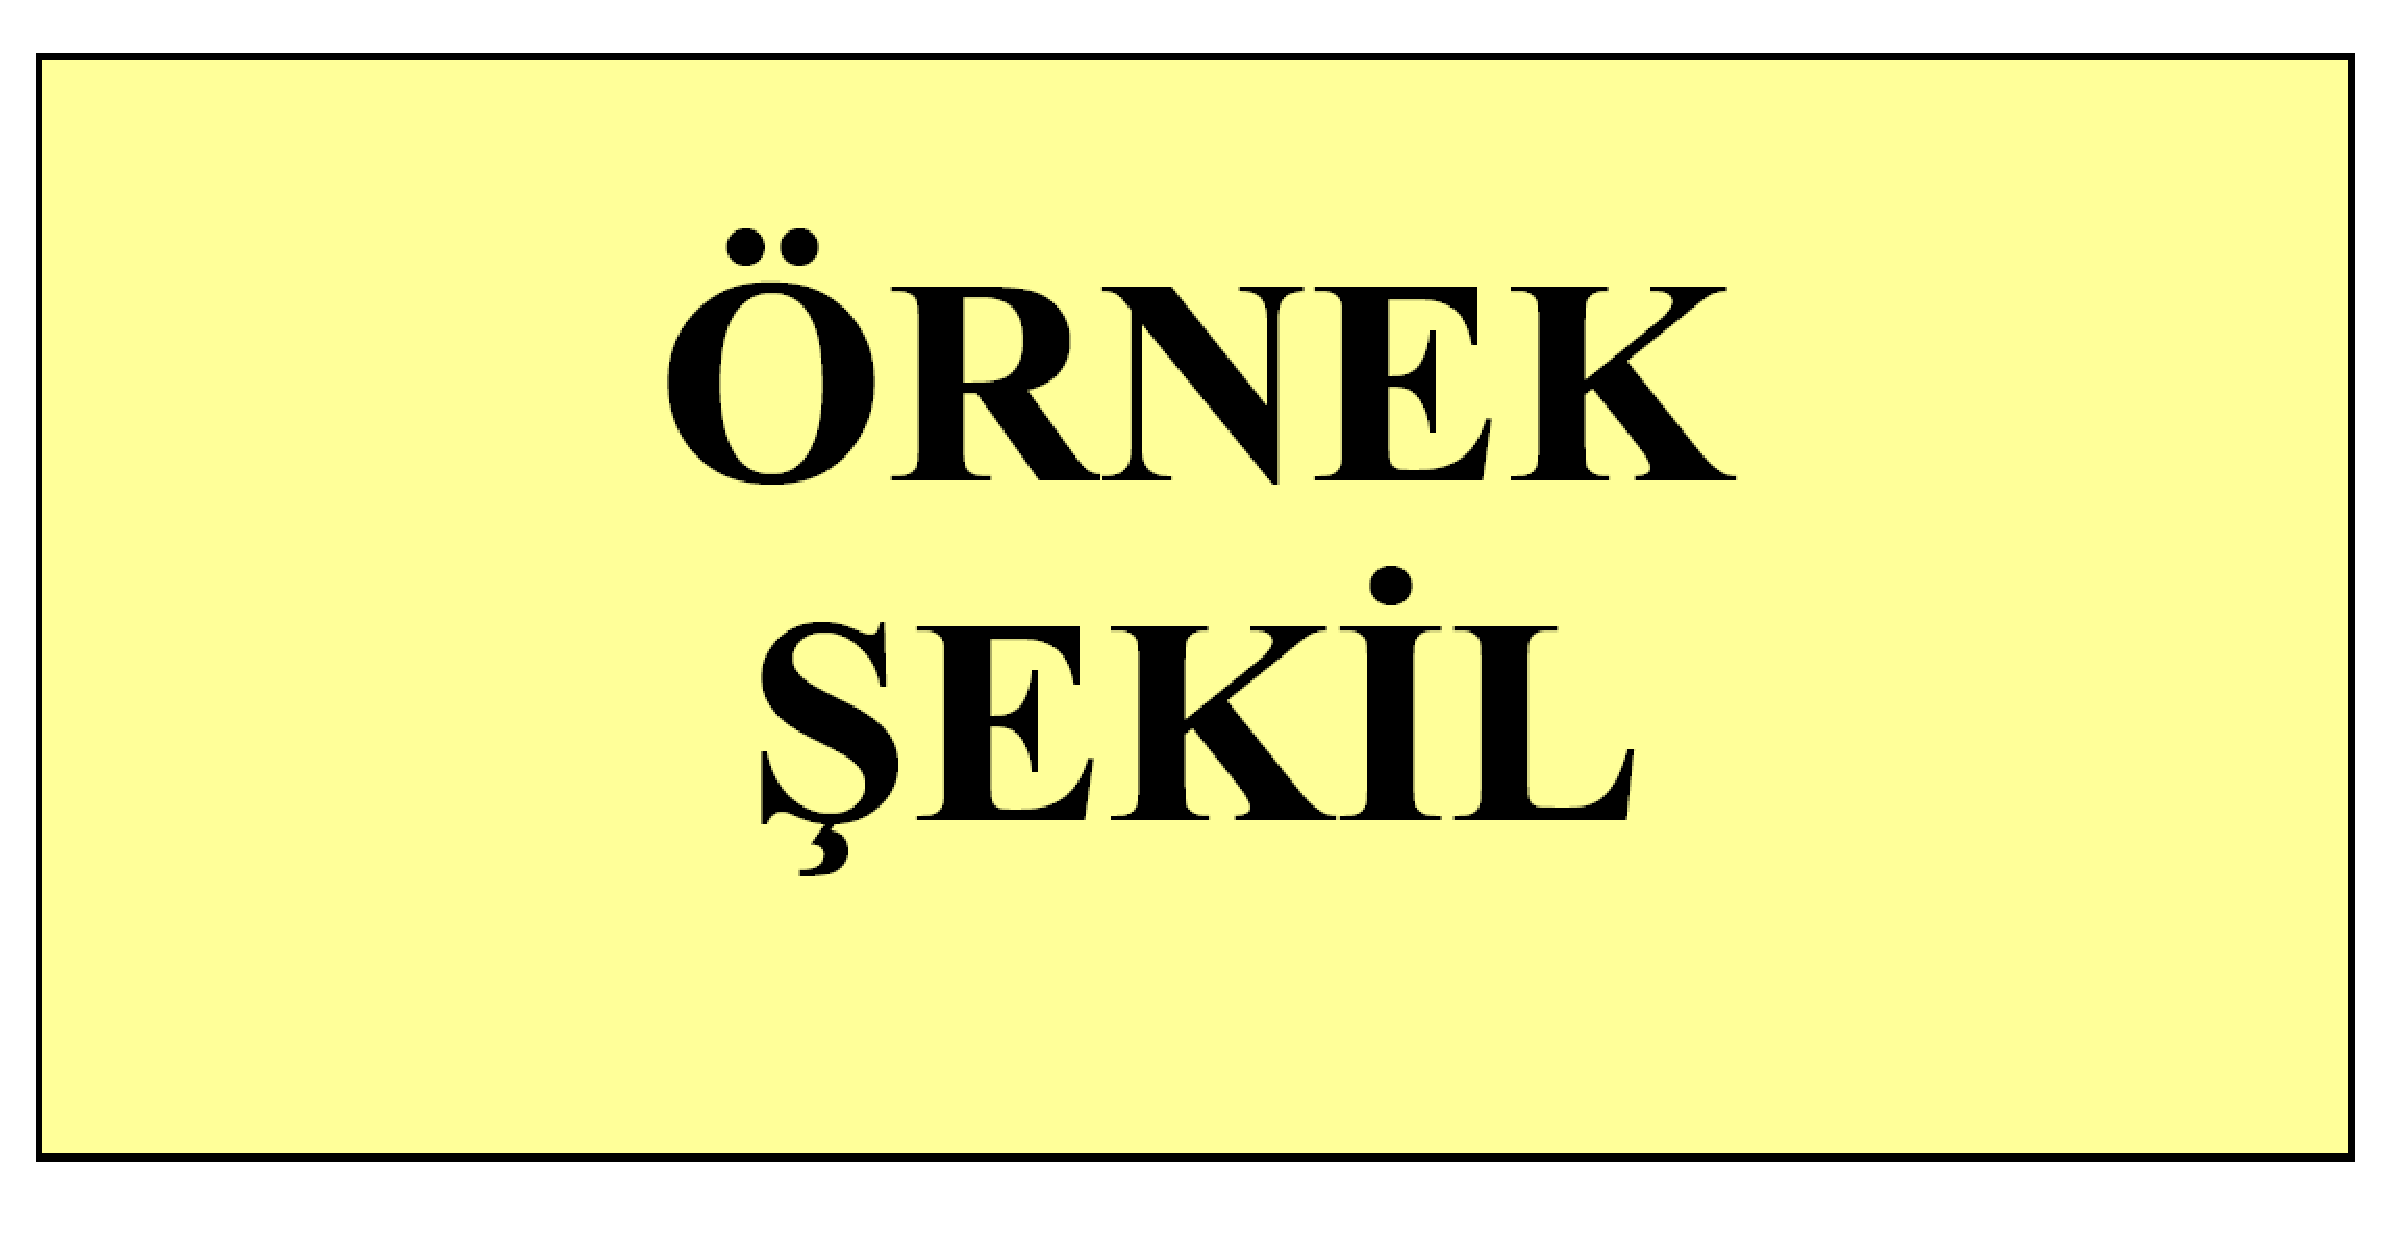
\includegraphics[width=250pt,keepaspectratio=true]{./fig/sekil4}
	% sekil4.eps: 0x0 pixel, 300dpi, 0.00x0.00 cm, bb=14 14 1148 603
	\caption{Figure captions must be ended with a full stop.}
	\label{Figure3.4}
\end{figure}

Lorem ipsum dolor sit amet, consetetur sadipscing elitr, sed diam nonumy eirmod tempor invidunt ut labore et dolore magna aliquyam erat, sed diam voluptua. Lorem ipsum dolor sit amet, consetetur sadipscing elitr, sed diam nonumy eirmod tempor invidunt ut labore et dolore magna aliquyam erat, sed diam voluptua. At vero eos et accusam et justo duo dolores et ea rebum. 
\begin{equation}
D\left(C_{A},C_{B}\right) = \min X_{A}\in C_{A},X_{B}\in C_{B} 
d\left(X_{A},X_{B}\right)
\label{Eq3.2}
\end{equation}
Lorem ipsum dolor sit amet, consetetur sadipscing elitr, sed diam nonumy eirmod tempor invidunt ut labore et dolore magna aliquyam erat, sed diam voluptua. Lorem ipsum dolor sit amet, consetetur sadipscing elitr, sed diam nonumy eirmod tempor invidunt ut labore et dolore magna aliquyam erat, sed diam voluptua. At vero eos et accusam et justo duo dolores et ea rebum. 

\section{Practical Applications}

Lorem ipsum dolor sit amet, consetetur sadipscing elitr, sed diam nonumy eirmod tempor invidunt ut labore et dolore magna aliquyam erat, sed diam voluptua. At vero eos et accusam et justo duo dolores et ea rebum. Stet clita kasd gub rgren, no sea takimata sanctus est Lorem ipsum dolor sit amet, consetetur sadipscing elitr, sed diam nonumy eirmod tempor invidunt ut lab ore sit et dolore magna.

Lorem ipsum dolor sit amet, consetetur sadipscing elitr, sed diam nonumy eirmod tempor invidunt ut labore et dolore magna aliquyam erat, sed diam voluptua. At vero eos et accusam et justo duo dolores et ea rebum. Stet clita kasd gub rgren, no sea takimata sanctus est Lorem ipsum dolor sit amet, consetetur sadipscing elitr, sed diam nonumy eirmod tempor invidunt ut lab ore sit et dolore magna.

\section{Application Data}

Lorem ipsum dolor sit amet, consetetur sadipscing elitr, sed diam nonumy eirmod tempor invidunt ut labore et dolore magna aliquyam erat, sed diam voluptua. At vero eos et accusam et justo duo dolores et ea rebum. Stet clita kasd gub rgren, no sea takimata sanctus est Lorem ipsum dolor sit amet, consetetur sadipscing elitr, sed diam nonumy eirmod tempor invidunt ut lab ore sit et dolore magna (Nelson, 1988).

Lorem ipsum dolor sit amet, consetetur sadipscing elitr, sed diam nonumy eirmod tempor invidunt ut labore et dolore magna aliquyam erat, sed diam voluptua. At vero eos et accusam et justo duo dolores et ea rebum. Lorem ipsum dolor sit amet, consetetur sadipscing elitr, sed diam nonumy eirmod tempor invidunt ut labore et dolore magna aliquyam erat, sed diam voluptua \cite{Wegener2000629}.

% ---------------------------------------------------------------- %
% Numbered citation.						                       %
% ---------------------------------------------------------------- %

Lorem ipsum dolor sit amet, consectetur adipiscing elit. Sed ac augue vel dui adipiscing placerat et nec metus \cite{Wolchik2000843}. 

Donec bibendum sodales mollis. Cras in lacus  justo, at vestibulum quam. Sed semper, est sit amet consectetur ornare, leo est lacinia velit, adipiscing elementum lectus felis at sem. Aenean hendrerit erat eu lacus malesuada at sodales arcu egestas. Maecenas euismod urna ut sem luctus et congue metus vulputate. Ut pellentesque, neque eget fringilla elementum, ligula massa aliquet lorem, et varius nisi lacus vel diam. Etiam vitae metus sed orci rutrum fringilla. Phasellus sed velit quam \cite{Zuckerman199486}. 

Mauris vestibulum, mauris a cursus adipiscing, nulla est hendrerit justo, ut fringilla eros velit ut mauris.

%%%%%%%%%%%%%%%%%%%%%%%%%%%%%%%%%%%%%%%%%%%%%%%%%%%%%%%%%%%%%%%%%
\chapter{REFERENCES, QUOTINGS AND FOOTNOTES}\label{Ch4}
%%%%%%%%%%%%%%%%%%%%%%%%%%%%%%%%%%%%%%%%%%%%%%%%%%%%%%%%%%%%%%%%%

In this section, information will be given about how citations, quotings and footnotes should be.

\section{Citing (indication of references in main text body)}

\subsection{Citing according to surname of author}

References are cited with the surname of author and year. In the references section, the references are listed alphabetically according to the surname of the author.

Citing of a reference at the beginning of or within a sentence must be as Boran (2003), whereas a citation at the end of a sentence must be as (Boran, 2003). The full-stop is placed directly after the citation.
 
A reference with two authors must be cited as Yılmaz and Johnson (2004) at the beginning of or within a sentence, or as (Yılmaz and Johnson, 2004) at the end of a sentence. 

A reference with more than two authors must be cited as Yılmaz et al. (2004) at the beginning of or within a sentence, or as (Yılmaz et al, 2004) at the end of a sentence. 

Different publications of an author published in the same year must be cited as Feray (2005a), Feray (2005b). 

While citing a part of a publication; the number of the page the cited material (chapter, table, figure, or equation) is on must be indicated. While citing, the expression “page” must be abbreviated, but “chapter” must not. For example; (Centers for Disease Control and Prevention, 2005, p. 10), (Shimamura, 1989, Chapter 3). 

Citing multiple publications in one pair of brackets; (Berndt, 2002; Harlow, 1983). 

Citing personal communication in main text body; (V.–G. Nguyen, personal communication, September 28, 1998), (J. Smith, personal communication, August 15, 2009).

In the references section, reference tags must be listed according to the surname of author. 

For citing of secondary references (In case the reference cites another reference), the secondary reference must be cited in brackets.  In the references section, the reference tag is organized according to the secondary reference, the original reference must not be used as a tag. For example; In his e-mails, Smith argued that asynchronous line dancing would be the next Internet meme (as cited in Jones, 2010).

\subsection{Citing according to order of appearance}

References are cited by numbering and indicating the number in square brackets ([]) in the main text body. The first reference cited in a thesis is numbered [1] and the following references are numbered according to the order of appearance. 

In the main text body, references must be cited as specified below:
\vspace*{-12pt}
\begin{tabbing}
\hspace*{1.5cm}\= \kill
[1]      \> Reference no. 1\\

[1--3]   \> References from no.1 to 3 (thus, references 1,2 and 3)\\

[1,3]    \> References no. 1 and 3\\

[1,3,8]  \> References no.1, 3 and 8\\

[1,3--8] \> References no.1, and from no.3 to 8 (thus, references 1, 3, 4, 5, 6, 7 and 8)
\end{tabbing}
\vspace*{-12pt}
Different volumes of a reference must be cited and numbered individually.

\section{Quoting}

Generally, quoting is done by remaining faithful to the original text in terms of words, spelling and punctuation. In case there is a mistake, the correct version is written in square brackets in the quoted text.

Short quotations (not longer than 40 words) must be given in quotation marks. Following the text quoted, the reference must be written and a full-stop must be placed afterwards.  

Quotations longer than 40 words must not be shown in quotation  marks. Instead, they must be indented 1 tab space (1.27 cm) from the left side of the page. The font size for long quotations indented from the left must be 2 pt smaller than the font size used in main text body. However, it is not advised to quote very long texts and to quote very frequently. Unlike short quotations, references of long quotations must be placed after the full stop. (i.e., .(p.196))

Example for a quotation at the beginning of a sentence;

According to Jones (1998), "Students often had difficulty using APA style,  especially when it was their first time" (p. 199).

Example for a quotation in the middle of a sentence;

Interpreting these results, Robbins et al. (2003) suggested that the “therapists in dropout cases may have inadvertently validated parental negativity about the adolescent without adequately responding to the adolescent’s needs or concerns” (p. 541) contributing to an overall climate of negativity.

Example for a quotation at the end of a sentence;

Confusing this issue is the overlapping nature of roles in palliative care, whereby “medical needs are met by those in the medical disciplines; nonmedical needs may be addressed by anyone on the team” (Csikai \& Chaitin, 2006, p. 112). 

Detailed information on quoting could be found on websites of Graduate Schools and associated links.

\section{Footnotes}

Footnotes could be used in theses to add content-expanding, content-enhancing, or additional information. 
Footnote numbers must be placed directly after a quotation. In case the quotation is a paragraph, the footnote numbers must be placed directly after the last word of the paragraph (as superscript). In case the quotation is a concept or a noun, footnote numbers must be placed directly after that concept or noun (as superscript). 

Footnote numbers in the main text body must be indicated as superscript, as shown\footnotemark. A punctuation mark must not be placed after the number.

Footnotes must be written with a font size 2 pt smaller than the main text body font size.
 
1 space must be set between footnote line and footnote number, 1/2 space must be set between footnote number and the first line of the footnote. Footnotes must be separated from the main text body with a thin horizontal line. 

Detailed information on footnotes could be found on the websites of Graduate Schools and associated links.

\footnotetext{~Reference display can not be done with footnotes.~Footnotes could be used in theses to add content-expanding, content-enhancing, or additional information.~If these information must include references, these references must be indicated in References section.}

\section{Second Level Title: First Letters Capital}

Lorem ipsum dolor sit amet, consetetur sadipscing elitr, sed diam nonumy eirmod tempor invidunt ut labore et dolore magna aliquyam erat, sed diam voluptua. At vero eos et accusam et justo duo dolores et ea rebum. Stet clita kasd gub rgren, no sea. 

\subsection{Third level title: Only first letter capital}

Lorem ipsum dolor sit amet, consetetur sadipscing elitr, sed diam nonumy eirmod tempor invidunt ut labore et dolore magna aliquyam erat, sed diam voluptua. At vero eos et accusam et justo duo dolores et ea rebum. Stet clita kasd gub rgren, no sea. 

\subsubsection{Fourth level title: Only first letter capital}

Stet clita kasd gub rgren, no sea takimata sanctus est Lorem ipsum dolor sit amet, consetetur sadipscing elitr, sed diam nonumy eirmod tempor invidunt ut lab ore sit et dolore magna.

\subsubsubsection{Fifth level title: No numbering after fourth level titles}

Stet clita kasd gub rgren, no sea takimata sanctus est Lorem ipsum dolor sit amet, consetetur sadipscing elitr, sed diam nonumy eirmod tempor invidunt ut lab ore sit et dolore magna\footnotemark.

% Include tilda to provide one letter spacing between the foot number and the text at the bottom - SBÖ
\footnotetext{~~Footnotes must be written with a font size 2 pt smaller than the main text body font size.}

\begin{figure}[t]
	\centering
	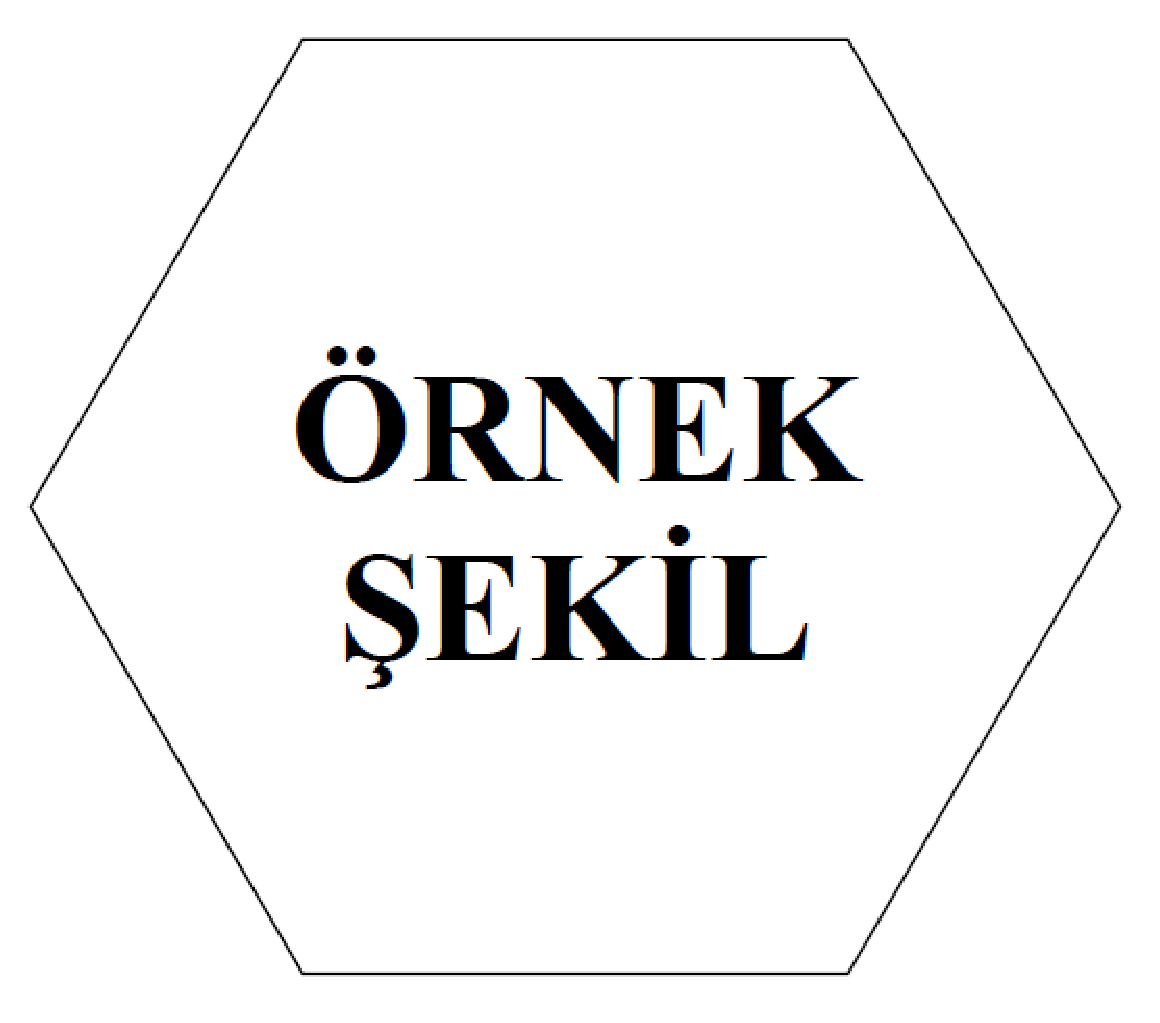
\includegraphics[width=230pt,keepaspectratio=true]{./fig/sekil6}
	% sekil6.eps: 0x0 pixel, 300dpi, 0.00x0.00 cm, bb=14 14 555 489
	\caption{Example figure.}
	\label{Figure4.1}
\end{figure}

This indicates that the ANN is accurate at base flow and flow height values lower then 3 m. 

\begin{table*}[h]
	{\setlength{\tabcolsep}{14pt}
		\caption{Example table.}
		\begin{center}
			\vspace{-6mm}
			\begin{tabular}{cccc}
				\hline \\[-2.45ex] \hline \\[-2.1ex]
				Column A & Column B & Column C & Column D \\
				\hline \\[-1.8ex]
				Row A & Row A & Row A & Row A \\
				Row B & Row B & Row B & Row B \\
				Row C & Row C & Row C & Row C \\
				[-0ex] \hline
			\end{tabular}
			\vspace{-6mm}
		\end{center}
		\label{Table4.1}}
\end{table*}

Stet clita kasd gub rgren, no sea takimata sanctus est Lorem ipsum dolor sit amet, consetetur sadipscing elitr, sed diam nonumy eirmod tempor invidunt ut lab ore sit et dolore magna. Stet clita kasd gub rgren, no sea takimata sanctus est Lorem ipsum dolor sit amet, consetetur sadipscing elitr, sed diam nonumy eirmod tempor invidunt ut lab ore sit et dolore magna.

Stet clita kasd gub rgren, no sea takimata sanctus est Lorem ipsum dolor sit amet, consetetur sadipscing elitr, sed diam nonumy eirmod tempor invidunt ut lab ore sit et dolore magna.  
%%%%%%%%%%%%%%%%%%%%%%%%%%%%%%%%%%%%%%%%%%%%%%%%%%%%%%%%%%%%%%%%%
\chapter{(IF NECESSARY) CHAPTER 5}\label{Ch5}
%%%%%%%%%%%%%%%%%%%%%%%%%%%%%%%%%%%%%%%%%%%%%%%%%%%%%%%%%%%%%%%%%

Lorem ipsum dolor sit amet, consetetur sadipscing elitr, sed diam nonumy eirmod tempor invidunt ut labore et dolore magna aliquyam erat, sed diam voluptua. At vero eos et accusam et justo duo dolores et ea rebum. Stet clita kasd gub rgren, no sea takimata sanctus est Lorem ipsum dolor sit amet, consetetur sadipscing elitr, sed diam nonumy eirmod tempor invidunt ut lab ore sit et dolore magna.

\section{Practical Application of This Study}

In this thesis, the necessary steps for constructing an end-to-end streamflow forecasting system were discussed. These steps include the use.

\section{Second Level Title: First Letters Capital}

Lorem ipsum dolor sit amet, consetetur sadipscing elitr, sed diam nonumy eirmod tempor invidunt ut labore et dolore magna aliquyam erat, sed diam voluptua. At vero eos et accusam et justo duo dolores et ea rebum. Stet clita kasd gub rgren, no sea.

\subsection{Third level title: Only first letter capital}

Lorem ipsum dolor sit amet, consetetur sadipscing elitr, sed diam nonumy eirmod tempor invidunt ut labore et dolore magna aliquyam erat, sed diam voluptua. At vero eos et accusam et justo duo dolores et ea rebum. Stet clita kasd gub rgren, no sea.

\subsubsection{Fourth level title: Only first letter capital}

Stet clita kasd gub rgren, no sea takimata sanctus est Lorem ipsum dolor sit amet, consetetur sadipscing elitr, sed diam nonumy eirmod tempor invidunt ut lab ore sit et dolore magna.

%\newpage
%{\bf Fifth level title: No numbering after fourth level titles}
\subsubsubsection{Fifth level title: No numbering after fourth level titles}

Lorem ipsum dolor sit amet, consetetur sadipscing elitr, sed diam nonumy eirmod tempor invidunt ut labore et dolore magna aliquyam erat, sed diam voluptua.

\begin{figure}
	\centering
	
\includegraphics[width=230pt,keepaspectratio=true]{./fig/sekil5}
	% sekil5.eps: 0x0 pixel, 300dpi, 0.00x0.00 cm, bb=14 14 1193 701
	\vspace{3mm}
	\caption{Example figure in chapter 5.}
	\label{Figure5.1}
\end{figure}

This indicates that the ANN is accurate at base flow and flow height values lower then 3 m. 

\begin{table*}[h]
	{\setlength{\tabcolsep}{14pt}
		\caption{Example table in chapter 5.}
		\begin{center}
			\vspace{-6mm}
			\begin{tabular}{cccc}
			    \hline \\[-2.45ex] \hline \\[-2.1ex]
				Column A & Column B & Column C & Column D \\
				\hline \\[-1.8ex]
				Row A & Row A & Row A & Row A \\
				Row B & Row B & Row B & Row B \\
				Row C & Row C & Row C & Row C \\
				[-0ex] \hline
			\end{tabular}
			\vspace{-6mm}
		\end{center}
		\label{Table5.1}}
\end{table*}

Stet clita kasd gub rgren, no sea takimata sanctus est Lorem ipsum dolor sit amet, consetetur sadipscing elitr, sed diam nonumy eirmod tempor invidunt ut lab ore sit et dolore magna. Stet clita kasd gub rgren, no sea takimata sanctus est Lorem ipsum dolor sit amet, consetetur sadipscing elitr, sed diam nonumy eirmod tempor invidunt ut lab ore sit et dolore magna.
 
Stet clita kasd gub rgren, no sea takimata sanctus est Lorem ipsum dolor sit amet, consetetur sadipscing elitr, sed diam nonumy eirmod tempor invidunt ut lab ore sit et dolore magna. Stet clita kasd gub rgren, no sea takimata sanctus est Lorem ipsum dolor sit amet, consetetur sadipscing elitr, sed diam nonumy eirmod tempor invidunt ut lab ore sit et dolore magna. 

%%%%%%%%%%%%%%%%%%%%%%%%%%%%%%%%%%%%%%%%%%%%%%%%%%%%%%%%%%%%%%%%%
\chapter{CONCLUSIONS AND RECOMMENDATIONS}\label{Ch6}
%%%%%%%%%%%%%%%%%%%%%%%%%%%%%%%%%%%%%%%%%%%%%%%%%%%%%%%%%%%%%%%%%

Lorem ipsum dolor sit amet, consetetur sadipscing elitr, sed diam nonumy eirmod tempor invidunt ut labore et dolore magna aliquyam erat, sed diam voluptua. At vero eos et accusam et justo duo dolores et ea rebum. Stet clita kasd gub rgren, no sea takimata sanctus est Lorem ipsum dolor sit amet, consetetur sadipscing elitr, sed diam nonumy eirmod tempor invidunt ut lab ore sit et dolore magna.

\section{Practical Application of This Study}

Lorem ipsum dolor sit amet, consetetur sadipscing elitr, sed diam nonumy eirmod tempor invidunt ut labore et dolore magna aliquyam erat, sed diam voluptua. At vero eos et accusam et justo duo dolores et ea rebum. Stet clita kasd gub rgren, no sea takimata sanctus est Lorem ipsum dolor sit amet, consetetur sadipscing elitr, sed diam nonumy eirmod tempor invidunt ut lab ore sit et dolore magna.

\section{Second Level Title: First Letters Capital}

Lorem ipsum dolor sit amet, consetetur sadipscing elitr, sed diam nonumy eirmod tempor invidunt ut labore et dolore magna aliquyam erat, sed diam voluptua. At vero eos et accusam et justo duo dolores et ea rebum. Stet clita kasd gub rgren, no sea.

\subsection{Third level title: Only first letter capital}

Lorem ipsum dolor sit amet, consetetur sadipscing elitr, sed diam nonumy eirmod tempor invidunt ut labore et dolore magna aliquyam erat, sed diam voluptua. At vero eos et accusam et justo duo dolores et ea rebum. Stet clita kasd gub rgren, no sea.

\subsubsection{Fourth level title: Only first letter capital}

Stet clita kasd gub rgren, no sea takimata sanctus est Lorem ipsum dolor sit amet, consetetur sadipscing elitr, sed diam nonumy eirmod tempor invidunt ut lab ore sit et dolore magna.

This indicates that the ANN is accurate at base flow and flow height values lower then 3 m. 

\begin{table*}[!htbp]
	{\setlength{\tabcolsep}{14pt}
		\caption{Example table in chapter 6.}
		\begin{center}
			\vspace{-6mm}
			\begin{tabular}{cccc}
				\hline \\[-2.45ex] \hline \\[-2.1ex]
				Column A & Column B & Column C & Column D \\
				\hline \\[-1.8ex]
				Row A & Row A & Row A & Row A \\
				Row B & Row B & Row B & Row B \\
				Row C & Row C & Row C & Row C \\
				[-0ex] \hline
			\end{tabular}
			\vspace{-6mm}
		\end{center}
		\label{Table6.1}}
\end{table*}

Stet clita kasd gub rgren, no sea takimata sanctus est Lorem ipsum dolor sit amet, consetetur sadipscing elitr, sed diam nonumy eirmod tempor invidunt ut lab ore sit et dolore magna. Stet clita kasd gub rgren, no sea takimata sanctus est Lorem ipsum dolor sit amet, consetetur sadipscing elitr, sed diam nonumy eirmod tempor invidunt ut lab ore sit et dolore magna. Stet clita kasd gub rgren, no sea takimata sanctus est Lorem ipsum dolor sit amet, consetetur sadipscing elitr, sed diam nonumy eirmod tempor invidunt ut lab ore sit et dolore magna. 

Stet clita kasd gub rgren, no sea takimata sanctus est Lorem ipsum dolor sit amet, consetetur sadipscing elitr, sed diam nonumy eirmod tempor invidunt ut lab ore sit et dolore magna. 

%{\bf Fifth level title: No numbering after fourth level titles}
\subsubsubsection{Fifth level title: No numbering after fourth level titles}

Lorem ipsum dolor sit amet, consectetur adipiscing elit. Sed ac augue vel dui adipiscing placerat et nec metus. Donec bibendum sodales mollis. Cras in lacus justo, at vestibulum quam. Sed semper, est sit amet consectetur ornare, leo est lacinia velit, adipiscing elementum lectus felis at sem.

\begin{figure}
	\centering
	
\includegraphics[width=230pt,keepaspectratio=true]{./fig/sekil7}
	% sekil7.eps: 0x0 pixel, 300dpi, 0.00x0.00 cm, bb=14 14 455 369
	\caption{Example table in chapter 6.}
	\label{Figure6.1}
\end{figure}

Lorem ipsum dolor sit amet, consectetur adipiscing elit. Sed ac augue vel dui adipiscing placerat et nec metus. Donec bibendum sodales mollis. Cras in lacus justo, at vestibulum quam. Sed semper, est sit amet consectetur ornare, leo est lacinia velit, adipiscing elementum lectus felis at sem.

Stet clita kasd gub rgren, no sea takimata sanctus est Lorem ipsum dolor sit amet, consetetur sadipscing elitr, sed diam nonumy eirmod tempor invidunt ut lab ore sit et dolore magna. Stet clita kasd gub rgren, no sea takimata sanctus est Lorem ipsum dolor sit amet, consetetur sadipscing elitr, sed diam nonumy eirmod tempor invidunt ut lab ore sit et dolore magna. Stet clita kasd gub rgren, no sea takimata sanctus est Lorem ipsum dolor sit amet, consetetur sadipscing elitr, sed diam nonumy eirmod tempor invidunt ut lab ore sit et dolore magna. 

Stet clita kasd gub rgren, no sea takimata sanctus est Lorem ipsum dolor sit amet, consetetur sadipscing elitr, sed diam nonumy eirmod tempor invidunt ut lab ore sit et dolore magna. 


% ----------------------------------------------------------------- %
% Form thesis_bib.bib to contain your references in bibtex format   %
% use \cite command for citing your references.                     %
% ----------------------------------------------------------------- %

\bibliographystyle{thesis_itubib}      % Designed .bst file 
\bibliography{thesis_bib}			   % .bib file

% ----------------------------------------------------------------- %
% Appendix files. appendices_cover is the appendix title page.      %
% ----------------------------------------------------------------- %

\eklerkapak{}
%\vglue18pt  % This has to be 18 pt - SBÖ
\singlespacing
\textbf{APPENDIX A.1 :} Example table and equations in the Appendices\\
\textbf{APPENDIX A.2 :} Additional information provided in the Appendices\\
\textbf{APPENDIX B.1 :} More additional information provided in the Appendices\\
\textbf{APPENDIX B.2 :} More and more additional information provided in the Appendices\\

One way of implementing multiple appendix in a row is to use itemize as in below to prevent issues on the indentation in the second line.

\begin{itemize}[leftmargin=3.3cm,itemsep=-0.4em,labelsep=1.5mm] % Adust margin to flush left, item sep., label sep. - SBÖ
\item [\textbf{APPENDIX A.1 :}]Example table and equations in the Appendices
\item [\textbf{APPENDIX A.2 :}]Additional information provided in the Appendices
\item [\textbf{APPENDIX B.1 :}]More additional information provided in the Appendices
\item [\textbf{APPENDIX B.2 :}]More and more additional information provided in the Appendices can go to the second line
\end{itemize}



\newpage

% ----------------------------------------------------------------- %
% \eklerbolum{x} forms and appendix of x chapters. 				    %
% ----------------------------------------------------------------- %

\eklerbolum{0}
\chapter{APPENDIX A.1}
\vglue6pt
% For Appendix A.1
% Format the equation environment
\renewcommand{\theequation}{A.1.\arabic{equation}}
% Reset the counter
\setcounter{equation}{0}

\begin{table*}[!ht]
	{\setlength{\tabcolsep}{14pt}
		\caption{Example table in appendix.}
		\begin{center}
			\vspace{-6mm}
			\begin{tabular}{cccc}
				\hline \\[-2.45ex] \hline \\[-2.1ex]
				Column A & Column B & Column C & Column D \\
				\hline \\[-1.8ex]
				Row A & Row A & Row A & Row A \\
				Row B & Row B & Row B & Row B \\
				Row C & Row C & Row C & Row C \\
				[-0ex] \hline
			\end{tabular}
			\vspace{-6mm}
		\end{center}
		\label{TableA.1}}
\end{table*}

\begin{equation}
y_{t} = \phi_{1} y_{t-1} + \epsilon_{t}
\label{EqA.1.1}
\end{equation}

Each parameter is described. As seen in equation \eqref{EqA.1.1}, or in \ref{EqA.1.1}.

\begin{equation}
y_{t} = \phi_{1} y_{t-1} + \epsilon_{t}
\label{EqA.1.2}
\end{equation}

\vspace*{12pt}

\section*{APPENDIX A.2}
\vglue6pt
% For Appendix A.2
% Format the equation environment
\renewcommand{\theequation}{A.2.\arabic{equation}}
% Reset the counter
\setcounter{equation}{0}

Lorem ipsum dolor sit amet, consectetur adipiscing elit. Sed ac augue vel dui adipiscing placerat et nec metus. Donec bibendum sodales mollis. Cras in lacus justo, at vestibulum quam. Sed semper, est sit amet consectetur ornare, leo est lacinia velit, adipiscing elementum lectus felis at sem.

\begin{equation}
y_{t} = \phi_{1} y_{t-1} + \epsilon_{t}
\label{EqA.2.1}
\end{equation}

Each parameter is described. As seen in equation \eqref{EqA.2.1}, or in \ref{EqA.2.1}.

\newpage

\chapter{APPENDIX B.1}
\vglue12pt
% For Appendix B.1
% Format the equation environment
\renewcommand{\theequation}{B.1.\arabic{equation}}
% Reset the counter
\setcounter{equation}{0}

Lorem ipsum dolor sit amet, consectetur adipiscing elit. Sed ac augue vel dui adipiscing placerat et nec metus. Donec bibendum sodales mollis. Cras in lacus justo, at vestibulum quam. Sed semper, est sit amet consectetur ornare, leo est lacinia velit, adipiscing elementum lectus felis at sem.

\begin{equation}
y_{t} = \phi_{1} y_{t-1} + \epsilon_{t}
\label{EqB.1.1}
\end{equation}
Each parameter is described. As seen in equation \eqref{EqB.1.1}, or in \ref{EqB.1.1}.

\begin{equation}
y_{t} = \phi_{1} y_{t-1} + \epsilon_{t}
\label{EqB.1.2}
\end{equation}

Each parameter is described. As seen in equation \eqref{EqB.1.2}, or in \ref{EqB.1.2}.

\begin{table*}[!ht]
	{\setlength{\tabcolsep}{14pt}
		\caption{Example table in appendix.}
		\begin{center}
			\vspace{-6mm}
			\begin{tabular}{cccc}
				\hline \\[-2.45ex] \hline \\[-2.1ex]
				Column A & Column B & Column C & Column D \\
				\hline \\[-1.8ex]
				Row A & Row A & Row A & Row A \\
				Row B & Row B & Row B & Row B \\
				Row C & Row C & Row C & Row C \\
				[-0ex] \hline
			\end{tabular}
			\vspace{-6mm}
		\end{center}
		\label{TableB.1}}
\end{table*}

\vspace*{18pt}

\section*{APPENDIX B.2}
\vglue6pt
% For Appendix B.2
% Format the equation environment
\renewcommand{\theequation}{B.2.\arabic{equation}}
% Reset the counter
\setcounter{equation}{0}

Lorem ipsum dolor sit amet, consectetur adipiscing elit. Sed ac augue vel dui adipiscing placerat et nec metus. Donec bibendum sodales mollis. Cras in lacus justo, at vestibulum quam. Sed semper, est sit amet consectetur ornare, leo est lacinia velit, adipiscing elementum lectus felis at sem.

\begin{equation}
y_{t} = \phi_{1} y_{t-1} + \epsilon_{t}
\label{EqB.2.1}
\end{equation}

Each parameter is described. As seen in equation \eqref{EqB.2.1}, or in \ref{EqB.2.1}.

\begin{table*}[!ht]
	{\setlength{\tabcolsep}{14pt}
		\caption{Example table in appendix.}
		\begin{center}
			\vspace{-6mm}
			\begin{tabular}{cccc}
				\hline \\[-2.45ex] \hline \\[-2.1ex]
				Column A & Column B & Column C & Column D \\
				\hline \\[-1.8ex]
				Row A & Row A & Row A & Row A \\
				Row B & Row B & Row B & Row B \\
				Row C & Row C & Row C & Row C \\
				[-0ex] \hline
			\end{tabular}
			\vspace{-6mm}
		\end{center}
		\label{TableB.2}}
\end{table*}


% ----------------------------------------------------------------- %
% The summary page                                                  %
% ----------------------------------------------------------------- %

\ozgecmis{\vspace*{10mm}
\setlength{\TPHorizModule}{10pt}
\setlength{\TPVertModule}{10pt}
\begin{textblock}{1}(43.25,15.75) % Photo is adusted flush to the right margin - SBÖ
	\begin{figure}[p]
		
\includegraphics[scale=0.35,keepaspectratio=true]{./fig/photo}
		% photo.eps: 0x0 pixel, 300dpi, 0.00x0.00 cm, bb=14 14 279 359
	\end{figure}	
\end{textblock}
\vspace*{30mm}
\textbf{Name Surname\makebox[2.155cm]{\hfill \textbf{:}}}\hspace{0.225em} \\ % Adjust the colomn alignment - SBÖ

\vspace{-3mm}
\textbf{Place and Date of Birth\makebox[0.735cm]{\hfill \textbf{:}}}\hspace{0.225em} \\ % Adjust the colomn alignment - SBÖ

\vspace{-3mm}
\textbf{E-Mail\makebox[3.685cm]{\hfill \textbf{:}}}\hspace{0.225em} \\ % Adjust the colomn alignment - SBÖ

\vspace{5mm}

\renewcommand\labelitemi{\normalsize$\bullet$} 			% Adjust the size of the bullets - SBÖ

\textbf{EDUCATION\makebox[2.41cm]{\hfill \textbf{:}}}  	% Adjust the colomn alignment - SBÖ
\vspace{-3mm}

\begin{itemize}[leftmargin=5.15cm,itemsep=-0.25em,labelsep=2mm] % Adjust margin to flush left, item sep., label sep. - SBÖ
	\item [$\bullet$ \hspace{1em}\textbf{B.Sc.} \hspace{6.85em} \textbf{:}] Graduation year, Istanbul Technical University, Faculty of Electrical and Electronics, Department of Electrical Engineering
	\item [$\bullet$ \hspace{1em}\textbf{M.Sc. \textcolor{red}{(If exists)}} \hspace{2.4em} \textbf{:}] Graduation year, Istanbul Technical University, Faculty of Electrical and Electronics, Department of Electrical Engineering
\end{itemize}

\textbf{PROFESSIONAL EXPERIENCE AND REWARDS:}   
\vspace{-3mm}
\begin{itemize}[leftmargin=0.7cm,itemsep=-0.25em,labelsep=5mm] % Adjust margin to flush left, item sep., label sep. - SBÖ
	%\setlength{\itemindent}{-0.25em}
	\item 1950-1956 Istanbul Technical University at the Central Laboratory of Theoretical Physics.
	\item 1953 Nobel Prize for Physics
	\item 1956 Completed Doctorate at Istanbul Technical University
\end{itemize}

\textbf{PUBLICATIONS, PRESENTATIONS AND PATENTS ON THE THESIS:} 
\vspace{-3mm}
\begin{itemize}[leftmargin=0.7cm,itemsep=0.5em,labelsep=5mm] % Adjust margin to flush left, item sep., label seperation - SBÖ
	%\setlength{\itemindent}{-0.25em}
	\item \textbf{Ganapuram S., Hamidov A., Demirel, M. C., Bozkurt E., Kındap U., Newton A.} % Bold authors font - SBÖ
	2007. Erasmus Mundus Scholar's Perspective On Water And Coastal
	Management Education In Europe. 
	\textit{International Congress - River Basin Management}, 
	March 22--24, 2007 Antalya, Turkey. \textcolor{red}{(Presentation Instance)}
	
	\item \textbf{Satoğlu, Ş.I., Durmuşoğlu, M. B., Ertay, T. A.} 2010. A Mathematical Model  % Bold authors font - SBÖ
	And A Heuristic Approach For Design Of The Hybrid Manufacturing Systems 
	To Facilitate One-Piece Flow, 
	\textit{International Journal of Production Research,}
	48(17), 5195--5220. \textcolor{red}{(Article Instance)}
	
	\item  \textbf{Chen, Z.} 2013. Intelligent Digital Teaching And Learning All-In-One Machine, % Bold authors font - SBÖ
	Has Projection Mechanism Whose Front End Is Connected With Supporting
	Arm, And Base Shell Provided With Panoramic Camera That Is Connected With
	Projector. Patent numarası: CN203102627-U. \textcolor{red}{(Patent Instance)}
\end{itemize}

%\newpage

\textbf{OTHER PUBLICATIONS, PRESENTATIONS AND PATENTS:} 
\vspace{-3mm}
% ---------------------------------------------------------------- %
% Fotografli ve yayin listeli (yayini varsa) ozgecmis onerilir.    %
% Fotograf ve adres sart degildir.				                   %
% ---------------------------------------------------------------- %

%======================================== SIRT OF THE THESIS ========================================= - SBÖ
\newpage % Last page is assigned for the SIRT of the Thesis 
\thispagestyle{empty} % Remove the bottom page number
% Definitions in sırt of the thesis
\def\sirtyili{2020} % Year of the graduation
\def\studentname{F. M. SURNAME} % F. and M. initials SURNAME
\def\thesisthickness{25mm} % Enter the expected thickness of the thesis after the hardcover 

\hspace*{75mm}
\begin{tikzpicture}[remember picture,overlay]
{\rotatebox[origin=c,x=23.35mm,y=-247.75mm]{90}{\draw [line width=0.01mm, black, dashed] (0mm,0mm) rectangle node{\normalsize \studentname} (65mm,\thesisthickness);}}

{\rotatebox[origin=c,x=23.35mm,y=-247.75mm]{90}{\draw [line width=0.01mm, black ,dashed, text width=190mm, align=center] (67mm,0mm) rectangle node{\normalsize \Baslikspacing \Baslikbir~\Baslikiki~\Baslikuc} (193mm+65mm+2mm,\thesisthickness);}}

{\rotatebox[origin=c,x=23.35mm,y=-247.75mm]{90}{\draw [line width=0.01mm, black ,dashed] (193mm+65mm+4mm,0mm) rectangle node{\normalsize \sirtyili} (296.5mm,\thesisthickness);}}

{\rotatebox[origin=c,x=23.35mm,y=-247.75mm]{90}{\draw[black,line width=1mm] (64.5mm,0mm) -- (64.5mm,\thesisthickness);
\draw[black,line width=1mm] (67.3mm,0mm) -- (67.3mm,\thesisthickness);
}}

{\rotatebox[origin=c,x=23.35mm,y=-247.75mm]{90}{\draw[black,line width=1mm] (193mm+64.5mm+2mm,0mm) -- (193mm+64.5mm+2mm,\thesisthickness);
\draw[black,line width=1mm] (193mm+64.5mm+5mm,0mm) -- (193mm+64.5mm+5mm,\thesisthickness);
}}
% Four dashed lines added between double thick lines vertically
\draw [line width=0.01mm, black, dashed] (0mm,-205mm) -- (0mm,-208mm);
\draw [line width=0.01mm, black, dashed] (-\thesisthickness,-205mm) -- (-\thesisthickness,-208mm);
\draw [line width=0.01mm, black, dashed] (0mm,-3.25mm) -- (0mm,-13mm);
\draw [line width=0.01mm, black, dashed] (-\thesisthickness,-1mm) -- (-\thesisthickness,-13mm);
\end{tikzpicture}} % Edge (Sırt) of the thesis at the very end.
\end{document}                      

% ----------------------------------------------------------------- %
% Updated voluntarily by	  :										%
% E. Baris Ondes    : ondes@itu.edu.tr 	  OR ondesalt@pm.me			% 
% Tamer Sener	    : senerta@itu.edu.tr  OR senertam@pm.me			%
% Berkan Kacmaz	    : kacmazb@itu.edu.tr  OR kacmazberkan0@gmail.com%
% S. Baris Ozturk   : ozturksb@itu.edu.tr OR salihbaris@gmail.com   %
% O. Ozgun Altunkaya: altunkayao@itu.edu.tr OR ozgun@pm.me 			%
% Latest update: 22-Feb-2021										%
% ----------------------------------------------------------------- %
